%%%%%%%%%%%%%%%%%%%%%%%%%%%%%%%%%%%%%%%%%%%%%%%%%%%%%%%
% Please note that whilst this template provides a 
% preview of the typeset manuscript for submission, it 
% will not necessarily be the final publication layout.
%
% letterpaper/a4paper: US/UK paper size toggle
% num-refs/alpha-refs: numeric/author-year citation and bibliography toggle


%\documentclass[letterpaper]{oup-contemporary}
\documentclass[a4paper,num-refs]{oup-contemporary}



%%% Journal toggle; only specific options recognised.
%%% (Only "gigascience" and "general" are implemented now. Support for other journals is planned.)%
%\journal{Test}
\jname{Università degli studi Roma Tor Vergata}
\jlogo{}

\usepackage{graphicx}
\usepackage{siunitx}
\usepackage{import}
\usepackage{amsmath}
%\numberwithin{equation}{section}% numera eq come #section.#formula
\usepackage{amsthm}
\usepackage{stmaryrd}
\usepackage{amssymb}
\usepackage{wasysym}
\usepackage{cancel}
\usepackage{textcomp}
\usepackage{cleveref}
\crefformat{section}{\S#2#1#3} % see manual of cleveref, section 8.2.1
\crefformat{subsection}{\S#2#1#3}
\crefformat{subsubsection}{\S#2#1#3}
\usepackage{lipsum}  
\usepackage{listings}
\definecolor{codegreen}{rgb}{0,0.6,0}
\definecolor{codegray}{rgb}{0.5,0.5,0.5}
\definecolor{codestring}{rgb}{0.4,0.4,0.4}
\definecolor{backcolour}{rgb}{0.96,0.96,0.96}
\definecolor{bbcolour}{rgb}{0.01,0.03,0.35}
\definecolor{indexcolour}{rgb}{0,0.4,0.4}
\lstdefinestyle{mystyle}{
	backgroundcolor=\color{backcolour},   
	commentstyle=\color{codegreen},
	classoffset=1,
	keywordstyle=\color{bbcolour},
	numberstyle=\tiny\color{codegray},
	stringstyle=\color{codestring},
	basicstyle=\ttfamily\small,
	breakatwhitespace=false,  
	breaklines=true,                 
	captionpos=b,                    
	keepspaces=false,                 
	numbers=left,                    
	numbersep=3pt,                  
	showspaces=false,                
	showstringspaces=false,
	showtabs=false,                  
	tabsize=2
}
\lstset{texcl=false, mathescape=true,style=mystyle}
\lstset{emph={%  
		i, j,X,n,Y%
	},emphstyle={\color{indexcolour}}%
}%

\usepackage[euler]{textgreek}


\usepackage{tikz}
\usetikzlibrary{shapes.geometric, arrows}
\tikzstyle{startstop} = [rectangle, rounded corners, minimum width=3cm, minimum height=1cm,text centered, draw=black, fill=backcolour]
\tikzstyle{startstop2} = [rectangle, rounded corners, minimum width=3cm, minimum height=2cm,text centered, draw=black, fill=backcolour]
\tikzstyle{io} = [trapezium, trapezium left angle=70, trapezium right angle=110, minimum width=2cm, minimum height=1cm, text centered,text width=2cm, draw=black, fill=backcolour]
\tikzstyle{io2} = [trapezium, trapezium left angle=70, trapezium right angle=110, minimum width=2cm, minimum height=1cm, text centered, draw=black, fill=backcolour]
\tikzstyle{process} = [rectangle, minimum width=3cm, minimum height=1cm, text centered,text width=4cm, draw=black, fill=backcolour]
\tikzstyle{decision} = [diamond, minimum width=2cm, minimum height=1cm, text centered, draw=black, fill=backcolour]
\tikzstyle{arrow} = [thick,->,>=stealth]
\tikzstyle{process2} = [rectangle, minimum width=2cm, text width=2cm,minimum height=1cm, text centered, draw=black, fill=backcolour]
\tikzstyle{process3} = [rectangle, minimum width=2cm,text width=2cm, minimum height=1cm, text centered, draw=black, fill=backcolour]


\definecolor{myred}{rgb}{0.545, 0.172, 0.031}
\usepackage[T1]{fontenc}
\usepackage[utf8]{inputenc}
\usepackage[italian, english]{babel}
\graphicspath{{figures/}} %Setting the graphicspat%h
\graphicspath{{figures/}} %Setting the graphicspath
\makeatletter
\providecommand*{\input@path}{}
\edef\input@path{{figures/}{}\input@path}% prepend
\makeatother


%%% Flushend: You can add this package to automatically balance the final page, but if things go awry (e.g. section contents appearing out-of-order or entire blocks or paragraphs are coloured), remove it!
% \usepackage{flushend}

\title{Omogeneizzazione numerica di materiali microstrutturati}

%%% Use the \authfn to add symbols for additional footnotes, if any. 1 is reserved for correspondence emails; then continuing with 2 etc for contributions.
\author{Mastrofini Alessandro}

%\affil[1]{First Institution}
%\affil[2]{Second Institution}

%%% Author Notes
\authnote{alessandro.mastrofini@alumni.uniroma2.eu}
%\authnote{\authfn{2}Contributed equally.}

%%% Paper category
\papercat{Meccanica Computazionale dei Tessuti e Biomateriali}

%%% "Short" author for running page header
\runningauthor{}

%%% Should only be set by an editor%
%\jvolume{00}
\jnumber{1}
\jyear{2021}

\begin{document}

\begin{frontmatter}
\maketitle
\begin{abstract}

Nel seguente report vengono introdotte diverse campagne di simulazione volte all'omogeneizzazione del tessuto osseo trabecolare. 
COMPLETE

COMPLETA

COMPLETAA


 \textbf{Background}, the context and purpose of the study;
 
  \textbf{Results}, the main findings;
  
   \textbf{Conclusions}, brief summary and potential implications. 
   
   Please minimize the use of abbreviations and do not cite references in the abstract.
\end{abstract}

\begin{keywords}
trabecular bone; homogenization; composite material
\end{keywords}
\end{frontmatter}



\section{Introduzione}

Lo scopo della seguente analisi è quello di indagare l'influenza delle proprietà microstrutturali sul comportamento macroscopico di un materiale composito.

Il flusso logico delle campagne di simulazioni è riportato in \cref{fig:flowchart}. 

Si parte dall'analizzare la struttura dell'osso trabecolare arrivando ad un volume rappresentativo idealizzato con una geometria tale da rispettare il rapporto tra i pori e la massa ossea trabecolare. Viene quindi discretizzato il RVE e il passaggio successivo prevede di ottimizzare la mesh in modo tale da avere un risultato sufficientemente accurato riducendo le richieste di sforzo computazionale. 

Si ottiene quindi una prima matrice di omogenizzazione che rispecchia le proprietà strutturali del RVE e dell'osso trabecolare così idealizzato. 

Vengono poi analizzate diverse proprietà geometriche e materiali seguendo le risposte dell'osso al carico, fenomeno noto come adattamento e rimodellamento osseo. 

\section{Tessuto osseo}

Il tessuto osseo è una forma specializzata di tessuto connettivo caratterizzata dalla mineralizzazione della matrice extracellulare. Questo conferisce al tessuto una notevole durezza e resistenza. È un tessuto in continua evoluzione, continuamente rinnovato e rimodellato per tutta la durata della vita. Costituisce l'impalcatura dello scheletro, da inserzione a muscoli e tendi e al suo interno contiene midollo osseo. 

Il tessuto osseo è costituito da cellule e da una matrice extracellulare, organica ed inorganica. La parte organica contiene fibre collagene e sostanza amorfa formata da glicoproteine e proteoglicani. 

Si possono distinguere due tipologie di osso: osso compatto e osso spugnoso \citep{Monesi}. 
L'osso compatto appare, all'esame macroscopico, come una singola massa solida. L'osso spugnoso invece ha un aspetto alveolare ed è costituito da sottili trabecole, che si anastomizzano in una rete tridimensionale. All'interno delle maglie che si formano con le spine trabecolari vi è accolto il midollo osseo.






ESCRIVI OSSO TRABECOLARE DA COWIN e LIBRO ISTOLOGIA

DESCRIVI BREVEMENTE PROPRIETà MECCANICHE NOTE DALLA LETTERATURA

TIPO:

Inoltre, è noto in letteratura che il parametro fondamentale e più influente nel legare la microstruttura alla risposta di rigidezza è la frazione volumetrica di pori. INSERISCI CITAZIONI

Ci sono però anche altri aspetti. Bisogna tenere conto che l'osso è un tessuto biologico e quindi soggetto al rimodellamento. In particolare è noto che l'osso risponde molto bene a stimoli di compressione andando ad aumentare la sua sezione trasversa ed inspessendo lo strato di osso compatto. Anche nell'osso spugnoso si vedono alcuni cambiamenti tra cui l'allineamento delle trabecole lungo le linee di forza.  \citep{Ferguson:2003}


\begin{figure*}%[b!]  %% Add a [b!] if you prefer the wide image to be at the bottm of the page
	\centering
	\def\svgwidth{\textwidth}
	\input{homogen.pdf_tex}
	\caption{Idealizzazione del RVE. (a) Ricostruzione tridimensionale; (b) Slice di riferimento no. 650; (c) ingrandimento del volume di interesse; (d) idealizzazione geometrica} 
	
\label{fig:homogen_RVE}
\end{figure*}
\begin{figure}[b!]
\begin{tikzpicture}
	\label{fig:flusso logico}
	\node (start) [startstop] {Osso trabecolare};
	\node (in1) [io, below of=start, yshift=-0.5cm] {Idealizzazione RVE};
	
	\node (pro1) [process, below of=in1, yshift=-1cm] {Omogenizzazione:
		\begin{itemize}
			\item condizioni al contorno
			\item soluzione FEM
			\item average stress
		\end{itemize}
	};
	\node (out1) [io2, below of=pro1, yshift=-1cm] {$\mathbb C^{(om)}$};
	\node (conv) [decision, below of=out1, yshift=-1.5cm] {Convergenza};
	
	\node (export) [startstop2, below of=conv, yshift=-2cm] {$\mathbb C^{(om)}=
		\begin{pmatrix}
			C_{11}&C_{12}&\cdot\\
			C_{21}&C_{22}&\cdot\\
			\cdot&\cdot&C_{66}
		\end{pmatrix}
		$};
	\node (pro2a) [process3, left of=conv, xshift=- 2.2cm] {Variazioni:
		\begin{itemize}
			\item geometria
			\item proprietà materiali
			\item finestra di interesse
	\end{itemize}};
	\node (pro2b) [process2, right of=conv, xshift=2cm] {Mesh};
	\draw [arrow] (start) -- (in1);
	\draw [arrow] (in1) -- (pro1);
	\draw [arrow] (pro1) -- (out1);
	\draw [arrow] (out1) -- (conv);
	\draw [arrow] (conv) -- (export);
	\draw [arrow] (conv) -- (pro2b);
	\draw [arrow] (pro2b) |- (pro1);
	\draw [arrow] (pro2a) |- (export);
	\draw [arrow] (pro1) -| (pro2a);
\end{tikzpicture} 
\caption{Flusso logico della campagna di simulazione}
\label{fig:flowchart}
\end{figure}

\section{Struttura multiscala}


In questa analisi viene presa come riferimento una vertebra lombare, L3. Le considerazioni sono comunque estensibili a qualunque altro osso trabecolare ma i parametri materiali fanno riferimento a dati selezionati per vertebre lombari.  
Le vertebre lombari sono solo alcune delle 33-34 vertebre che formano la colonna vertebrale umana. Il corpo vertebrale è formato principalmente da osso trabecolare con le singole trabecole allineate lungo le linee di forza. Questa disposizione fornisce un contributo importante per la distribuzione dei carichi e il sostegno del busto. Circa tre quarti dell'intero carico strutturale ricadono sulla colonna anteriore, ovvero sul corpo vertebrale, dischi intervertebrali e sulle placche terminali delle vertebre. La struttura ossea trabecolare può subire diversi cambiamenti con l'invecchiamento o a causa di alcune patologie \citep{Ferguson:2003} come la perdita di densità minerale, cambiamenti morfologici come un aumento della frazione volumetrica di pori, ispessimento o assottigliamento delle trabecole e perdita di connettività. Questi cambiamenti influenzano notevolmente la risposta meccanica del tessuto. 

L'osso è composto da diverse fasi. Contiene una fase organica, una inorganica e acqua. La fase organica è composta da collagene e proteine mentre la fase inorganica da fosfato di calcio, simile all'idrossiapatite \citep{Hamed:2012}. Alla nanoscala si trovano le molecole di collagene e i cristalli di idrossiapatite. Si passa poi ad una scala leggermente maggiore dove delle fibrille mineralizzate si uniscono a formare una singola lamella di spessore alcuni $\mu m$. Le singole lamelle si impacchettano a formare delle trabecole con uno spessore medio di 50$\mu m$ e una lunghezza di circa 1mm. Siamo alla microscala. Si passa poi ad una scala intermedia dove possiamo considerare il volume di interesse di questa analisi dove troviamo sia trabecole che i pori riempiti di midollo fino ad arrivare alla macroscala dove si guarda all'osso nel suo insieme. 

L'obiettivo della seguente analisi è quello di portare in conto le differenze alla microscala, considerando un volume rappresentativo, e omogenizzare le proprietà meccaniche ottenendo un'unica matrice di rigidezza omogenizzata.    








\section{Omogenizzazione}

L'obiettivo è quindi quello di ottenere delle proprietà materiali alla macroscala a partire dalle proprietà alla microscala come le rigidezza dei due materiali, matrice ossea e pori.

Ad una sclaa sufficientemente grande rispetto le singole trabecolee è possibile considerare la matrice di midollo e le trabecole ossee come due materiali diversi ma entrambi eterogenei e dal comportamento isotropo. L'isootropia è una prima approssimazione che però ci permette di procedere in modo più efficiente nell'omogenizzazione andando a vedere come la struttura e la disposizione dei pori influenzi il comportamento macroscopico. 

Con la procedura di omogenizzazione andremo a considerare una media delle proprietà meccaniche di osso e matrice ma questa media viene intesa in senso più ampio e il significato può variare a seconda dell'approccio. 

\subsection{Volume di interesse}
\label{sec:RVE}

Il primo passo, per poter procedere ad un'omogenizzazione, è quello di definire un volume rappresentativo (RVE) tale da essere rappresentativo dal punto di vista statistico della distribuzione geometrica dei costituenti, quindi della microscala. Per farlo il codice calcola automaticamente il lato nel range di qualche mm a partire da alcune considerazioni. Viene rispettato il diametro medio dei pori \citep{Doktor:2011} e la frazione volumetrica  \citep{Cowin1}. 

Sulla base di queste considerazioni vengono inseriti 25 pori equidistanti e tali che la loro distanza dal bordo sia la metà della distanza tra ogni poro. Questo consente di avere un RVE simmetrico e rappresentativo di una selezione delle trabecole. 

Maggiori informazioni sulla procedura di automazione del calcolo del RVE sono nella sezione \ref{sec:RVE_code}.

Inoltre, per fare le opportune considerazioni nel considerare le tensioni medie, i pori vengono considerati pieni di un materiale a bassa rigidezza rappresentativo del midollo osseo. Questo serve sia a considerare un fenomeno più rappresentativo della realtà sia a permettere una corretta applicazione del teorema della media delle tensioni. 




\subsection{Stime analitiche}

Per confrontare i dati dell'omogenizzazione vengono considerate le stime analitiche di Voigt e Reuss. 

L'approssimazione di Voigt considera la matrice di rigidezza come una media pesata per le volume fraction delle rigidezze dei costituenti. 
\begin{equation}
	\mathbb C_{\operatorname{Voigt}}=(1-v_f)\mathbb C_b+v_f \mathbb C_m
\end{equation}

Le stime di Reuss sono analoghe ma in cedevolezza:

\begin{equation}
	\mathbb S_{\operatorname{Voigt}}=(1-v_f)\mathbb S_b+v_f \mathbb S_m
\end{equation}

Vengono considerate queste due stime per via del teorema di Hill che garantisce, sotto le opportune ipotesi, che la matrice di rigidezza sia compresa tra queste \citep{ABOUDI201387}. Reuss costituisce il limite inferiore e Voigt il limite superiore dell'omogenizzazione. 

I due materiali vengono con considerati singolarmente isotropi, quindi tali da avere un comportamento materiale descritto dalla matrice di cedevolezza  \eqref{eq:isotropic_S}.

\begin{equation}
[\mathbb S]_{\operatorname{iso}}=\left[\begin{array}{cccccc}
	\frac{1}{E} & -\frac{\nu}{E} & -\frac{\nu}{E} & 0 & 0 & 0 \\
	-\frac{\nu}{E} & \frac{1}{E} & -\frac{\nu}{E} & 0 & 0 & 0 \\
	-\frac{\nu}{E} & -\frac{\nu}{E} & \frac{1}{E} & 0 & 0 & 0 \\
	0 & 0 & 0 & \frac{2(1+\nu)}{E} & 0 & 0 \\
	0 & 0 & 0 & 0 & \frac{2(1+\nu)}{E} & 0 \\
	0 & 0 & 0 & 0 & 0 & \frac{2(1+\nu)}{E}
\end{array}\right]
\label{eq:isotropic_S}
\end{equation}

Queste matrici vengono calcolate e per ogni iterazione del processo di omogenizzazione viene verificato che il risultato sia compreso in tali stime tramite la funzione \texttt{VoigtReussTest[]}. In particolare, passando la variabile \texttt{verbOutput==True} è possibile estrarne i valori:
\begin{equation}
\mathbb C_{Voigt}=\begin{pmatrix}
	2019.340&865.404&0\\
	865.404&2019.340&0\\
	0&0&576.969
	
\end{pmatrix}
\end{equation}

\begin{equation}
	\mathbb C_{Reuss}=\mathbb S_{Reuss}^{-1}=\begin{pmatrix}
0.226262&0.0399292&0\\
0.0399292&0.226262&0\\
0&0&0.0931663
	\end{pmatrix}
\end{equation}


\subsection{Omogenizzazione numerica}
\label{sec:homogen}

Viene quindi strutturata una campagna di simulazioni tale da analizzare il RVE ed estrarre una matrice di rigidezza omogenizzata. Ulteriori considerazioni vengono fatte sul parametro $\mathbb C_{11}^{(om)}$.

L'approccio all'omogenizzazione segue condizioni al bordo omogenee di tipo spostamento.  
In particolare, applicheremo un campo di spostamento alla macroscala supponendo che sia rappresentativo di quello alla microscala. Quindi otterremo un certo campo di tensione alla microscala, funzione del punto. Possiamo quindi considerare il campo di tensione alla macroscala come la media di quello alla microscala. In particolare, queste condizioni sono garantite dall'Average Strain Theorem.
Quindi le tensioni medie misurate nel RVE sono definite come:
\begin{equation}
	\left< \boldsymbol{\sigma}\right> ={1\over \|\tilde \Omega\|}\int _{\tilde \Omega} \boldsymbol{\varepsilon} \:d\tilde \Omega
\end{equation}
dove $\tilde \Omega$ è l'area del RVE.

Applicando un campo di deformazione alla macroscala otterrei le deformazioni alla microscala e potrei estrarre le tensioni semplicemente risolvendo il problema dell'equilibrio elastico:
\begin{equation}
\boldsymbol{\sigma}=\tilde{\left<{\boldsymbol{\sigma}}\right>}=\mathbb C\tilde{\left<{\boldsymbol{\varepsilon}}\right>}=\mathbb C \boldsymbol{\varepsilon}
\end{equation}
In particolare, applicando condizioni di deformazione unitaria su $\varepsilon_1$,$\varepsilon_2$ e $\gamma_{12}$ otterrei rispettivamente prima, seconda e terza colonna di $\mathbb C$. È possibile farlo in tre processi carico separati e considerare il contributo complessivo in quanto siamo in elasticità lineare sotto l'ipotesi di piccole deformazioni per cui vale la sovrapposizione degli effetti.

DESCRIVI IL METODO FEM 

Questo viene implementato tramite una campagna di simulazioni in \texttt{Mathematica} sfruttando il tool \texttt{AceFEM}. 

Viene sfruttata la procedura \texttt{TEST[]} che permette di applicare in sequenza le tre condizioni di spostamento e ottenere così la matrice di rigidezza:

\begin{equation}
\mathbb C^{(om)}=\left(
\begin{array}{ccc}
	756.78 & 80.90 & 0.00 \\
	80.90 & 756.78 & 0.00 \\
	0.00 & 0.00 & 40.87\\
\end{array}
\right)
\end{equation}.

Da questa matrice è possibile innanzitutto verificare che sono soddisfatti i limiti inferiore e superiore (Reuss e Voigt). 
Si vede inoltre un comportamento isotropo e come l'elevata pore fraction e quindi la grande presenza di materiale a bassa rigidezza va ad abbassare la rigidezza della matrice ossea. 

Ulteriori informazioni sull'automazione e sulla convergenza di questo risultato sono presenti nella sezione dell'analisi a convergenza \cref{sec:convergenza}.


\begin{table}[bt!]
	\caption{Parametri materiali}\label{tab:example}
	\begin{tabular}{l r l}
		\toprule
		Nome & Valore &  Reference\\
		\midrule
		$E_b$ & $3.8$ GPa & \citet{Cowin1}  \\
		$\nu_b$  & $0.3$ & \citet{Dalstra:93,Wirtz:2000}  \\
		$E_m$  & $15$ KPa  & \citet{Jansen:2015} \\ 
		$\nu_m$ & $0.1 $&    \\
		
		$C_{11}^{(b)}$&$6730.77 $MPa& \cref{sec:homogen} \textsuperscript{*}\\
		$C_{11}^{(m)}$& $0.15$ Mpa& \cref{sec:homogen} \textsuperscript{*}\\
		$C_{11}^{(om)}$& $756.78 $ Mpa & \cref{sec:homogen} \textsuperscript{*}\\
		$L$ & $1.324$ mm& \cref{sec:RVE} \textsuperscript{*}\\
		\bottomrule
	\end{tabular}
	\begin{tablenotes}
		
		\item \textsuperscript{*}Parametri calcolati
	\end{tablenotes}
\end{table}


\section{Variazione della microstruttura}

Il carico della colonna vertebrale ricade per la maggior parte sul corpo vertebrale e sui dischi intervertebrali. Il corpo vetebrale è fornato da osso trabecolare ad alta porosità con un guscio esterno altamente denso. Tuttavia, il guscio esterno è molto sottile ed è formato da un addensamento di osso trabecolare molto compatto, istologicamente differente dall'osso corticale. Diverse analisi agli elementi finito hanno stimato che il guscio esterno contribuisce per meno del 15\% alla Capacità di carico globale della vertebra \citep{Ferguson:2003, Silva:1997}.

Inoltre, diversi campioni di osso trabecolare hanno mostrato diverse proprietà meccaniche a seconda della regione dove vengono prelevati. \citep{Keller:1989,Keller:1993}. Questo è segno della risposta dell'osso che, essendo un tessuto vivo e in continuo rimodellamento, è variabile e si adatta all'ambiente. L'aumento delle proprietà di resisitenza a compressione nella parte centrale dell'osso è di fatto un risposta al maggior carico verticale trasmesso dalla parte polposa del disco vertebrale rispetto all'adicente regione periferica di anelli fibrosi. 

Sulla base di queste considerazioni sono state condotte ulteriori analisi variando la geometria del RVE e osservando come varia la risposta materiale risultante. Le variazioni considerate seguono dall'idealizzazione di alcuni fenomeni fisiologici che portano al rimodellamento osseo indotto dall'ambiente meccanico in cui si trova.



\subsection{Variazione della simmetria}

\begin{figure*} 
	\centering
	\begin{minipage}[b]{0.19\linewidth}
		\centering
		$\operatorname{AxR}=0.8	$
	\end{minipage}
	\begin{minipage}[b]{0.19\linewidth}
		\centering
		$\operatorname{AxR}=0.6	$
	\end{minipage}
	\begin{minipage}[b]{0.19\linewidth}
		\centering
		$	\operatorname{AxR}=0.5$
	\end{minipage}
	\begin{minipage}[b]{0.19\linewidth}
		\centering
		$	\operatorname{AxR}=0.3$
	\end{minipage}
	\begin{minipage}[b]{0.19\linewidth}
		\centering
		$	\operatorname{AxR}=0.1$
	\end{minipage} 
	\begin{minipage}[b]{0.19\linewidth}
		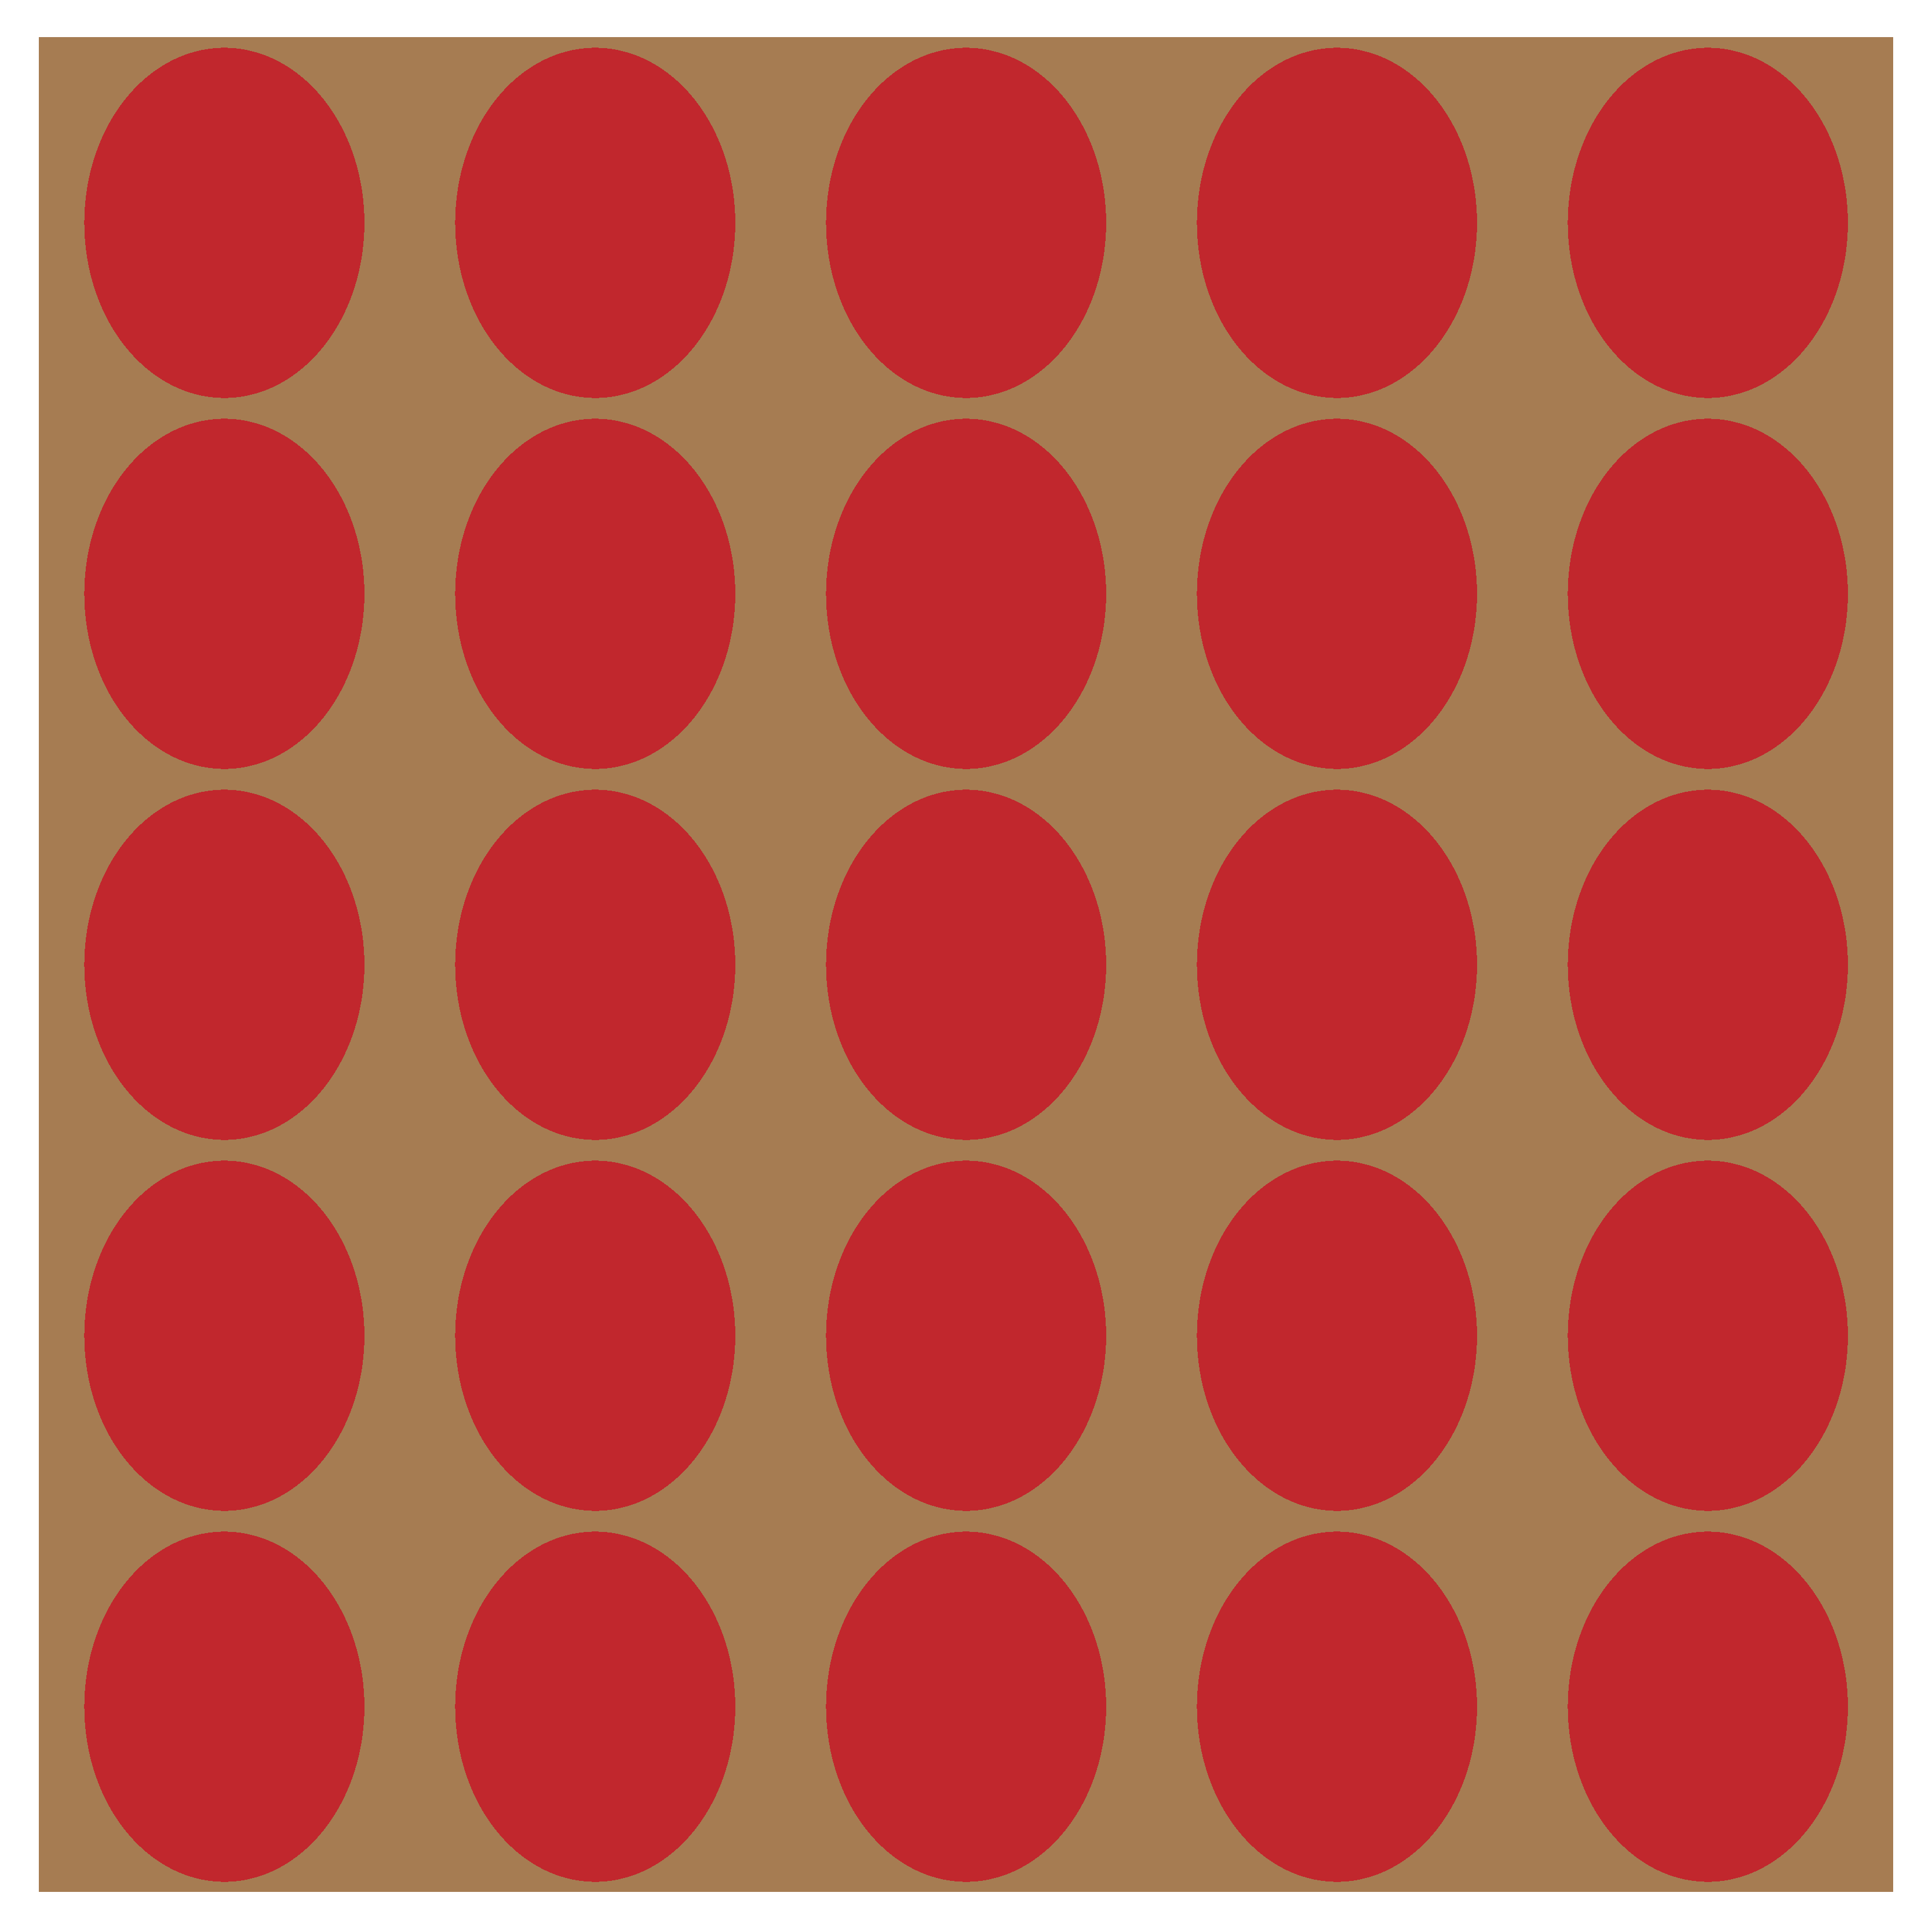
\includegraphics[width=\linewidth]{test_mesh_axR_0.8.png}
	\end{minipage} 
	\begin{minipage}[b]{0.19\linewidth}
		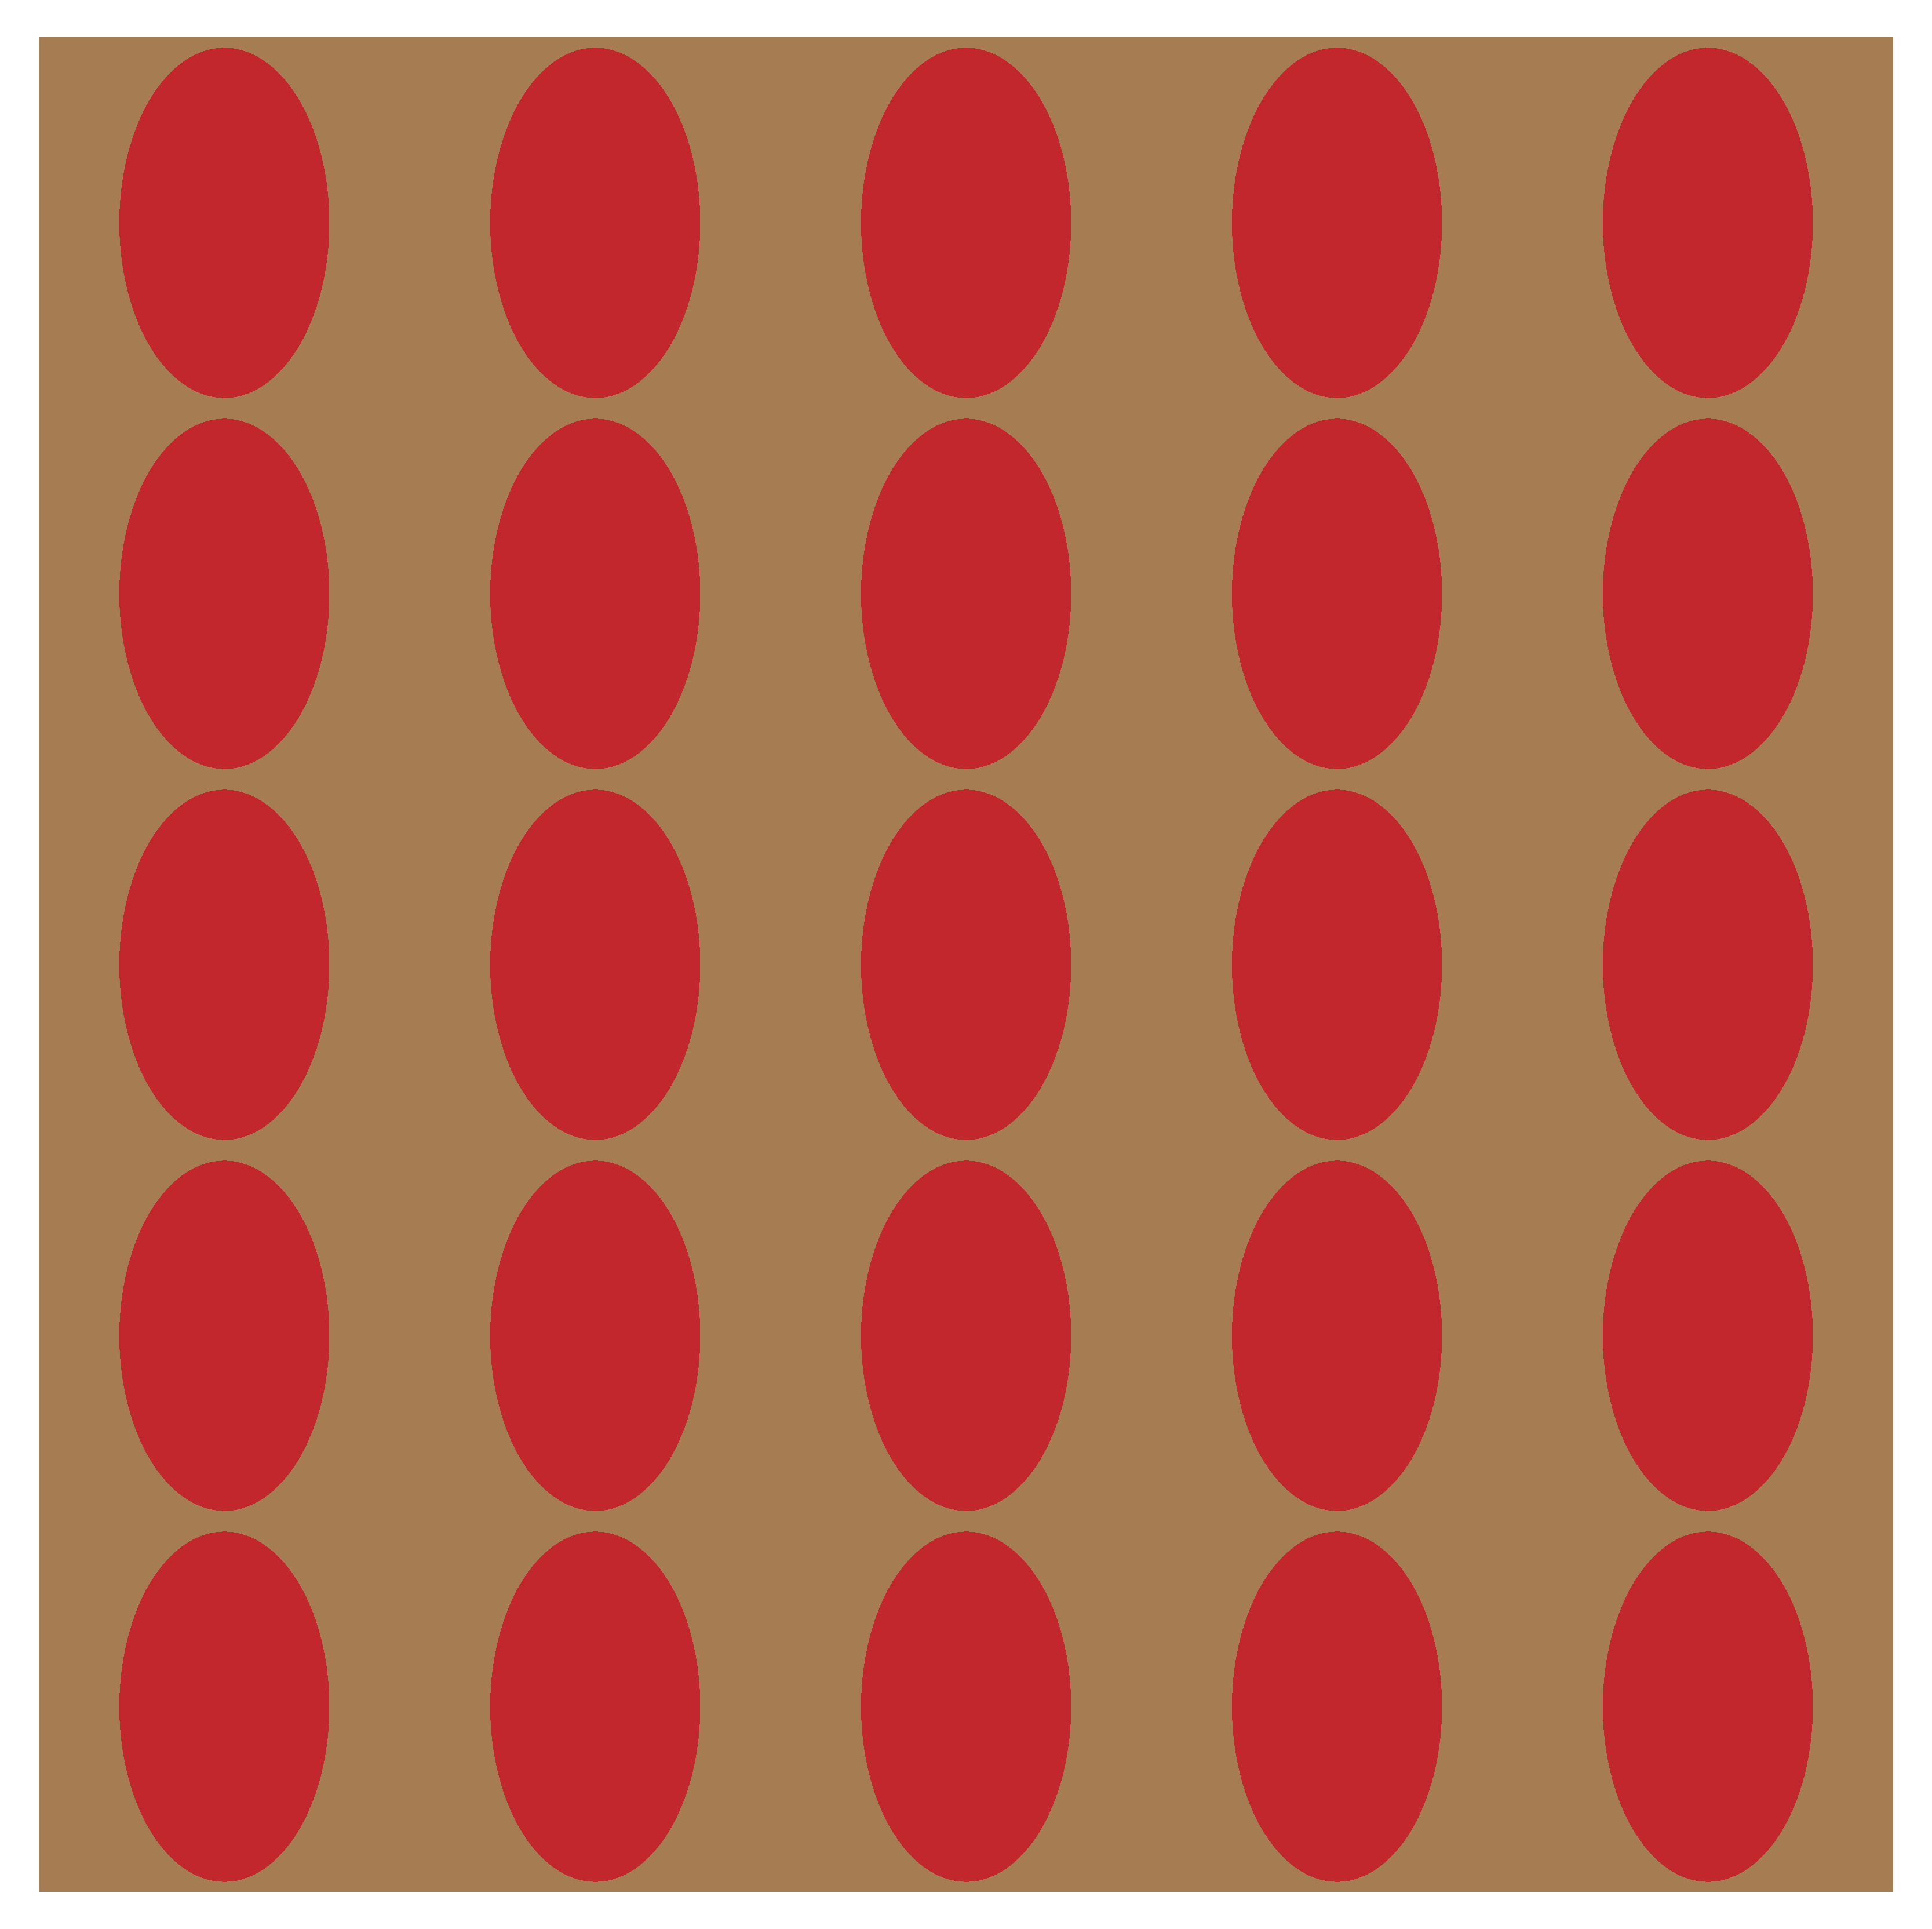
\includegraphics[width=\linewidth]{test_mesh_axR_0.6.png}
	\end{minipage} 
	\begin{minipage}[b]{0.19\linewidth}
		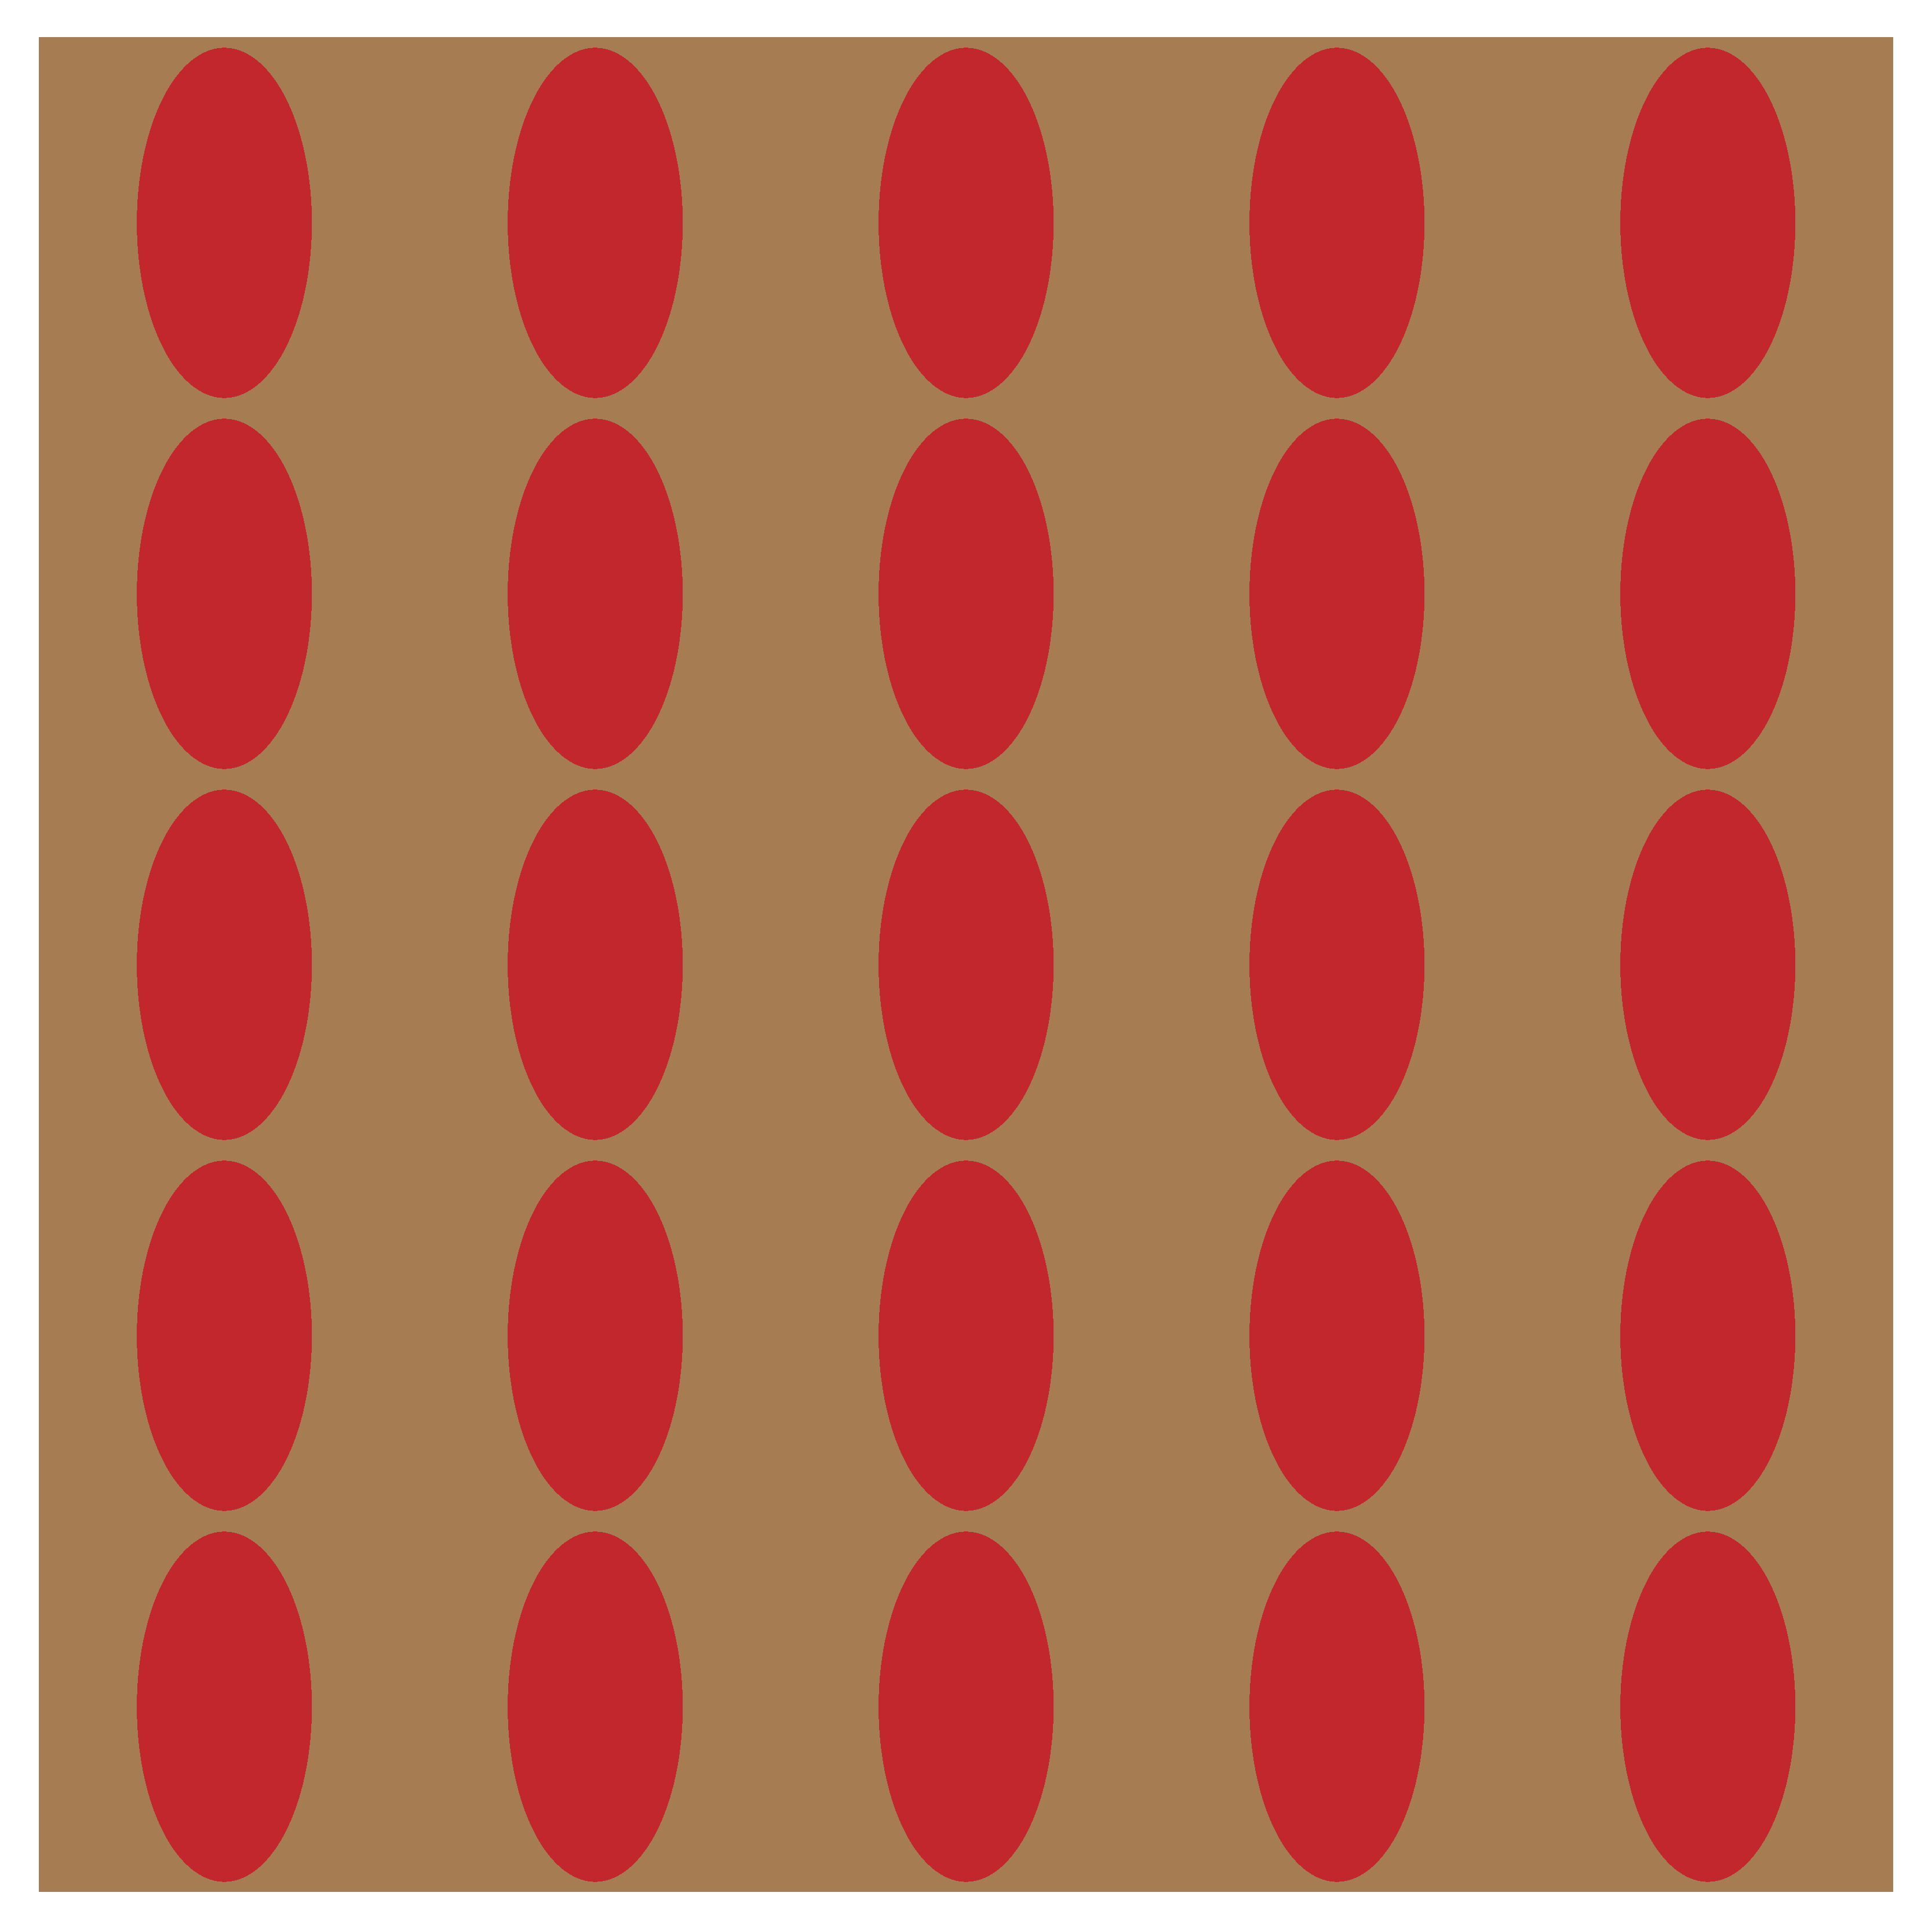
\includegraphics[width=\linewidth]{test_mesh_axR_0.5.png}
	\end{minipage}
	\begin{minipage}[b]{0.19\linewidth}
		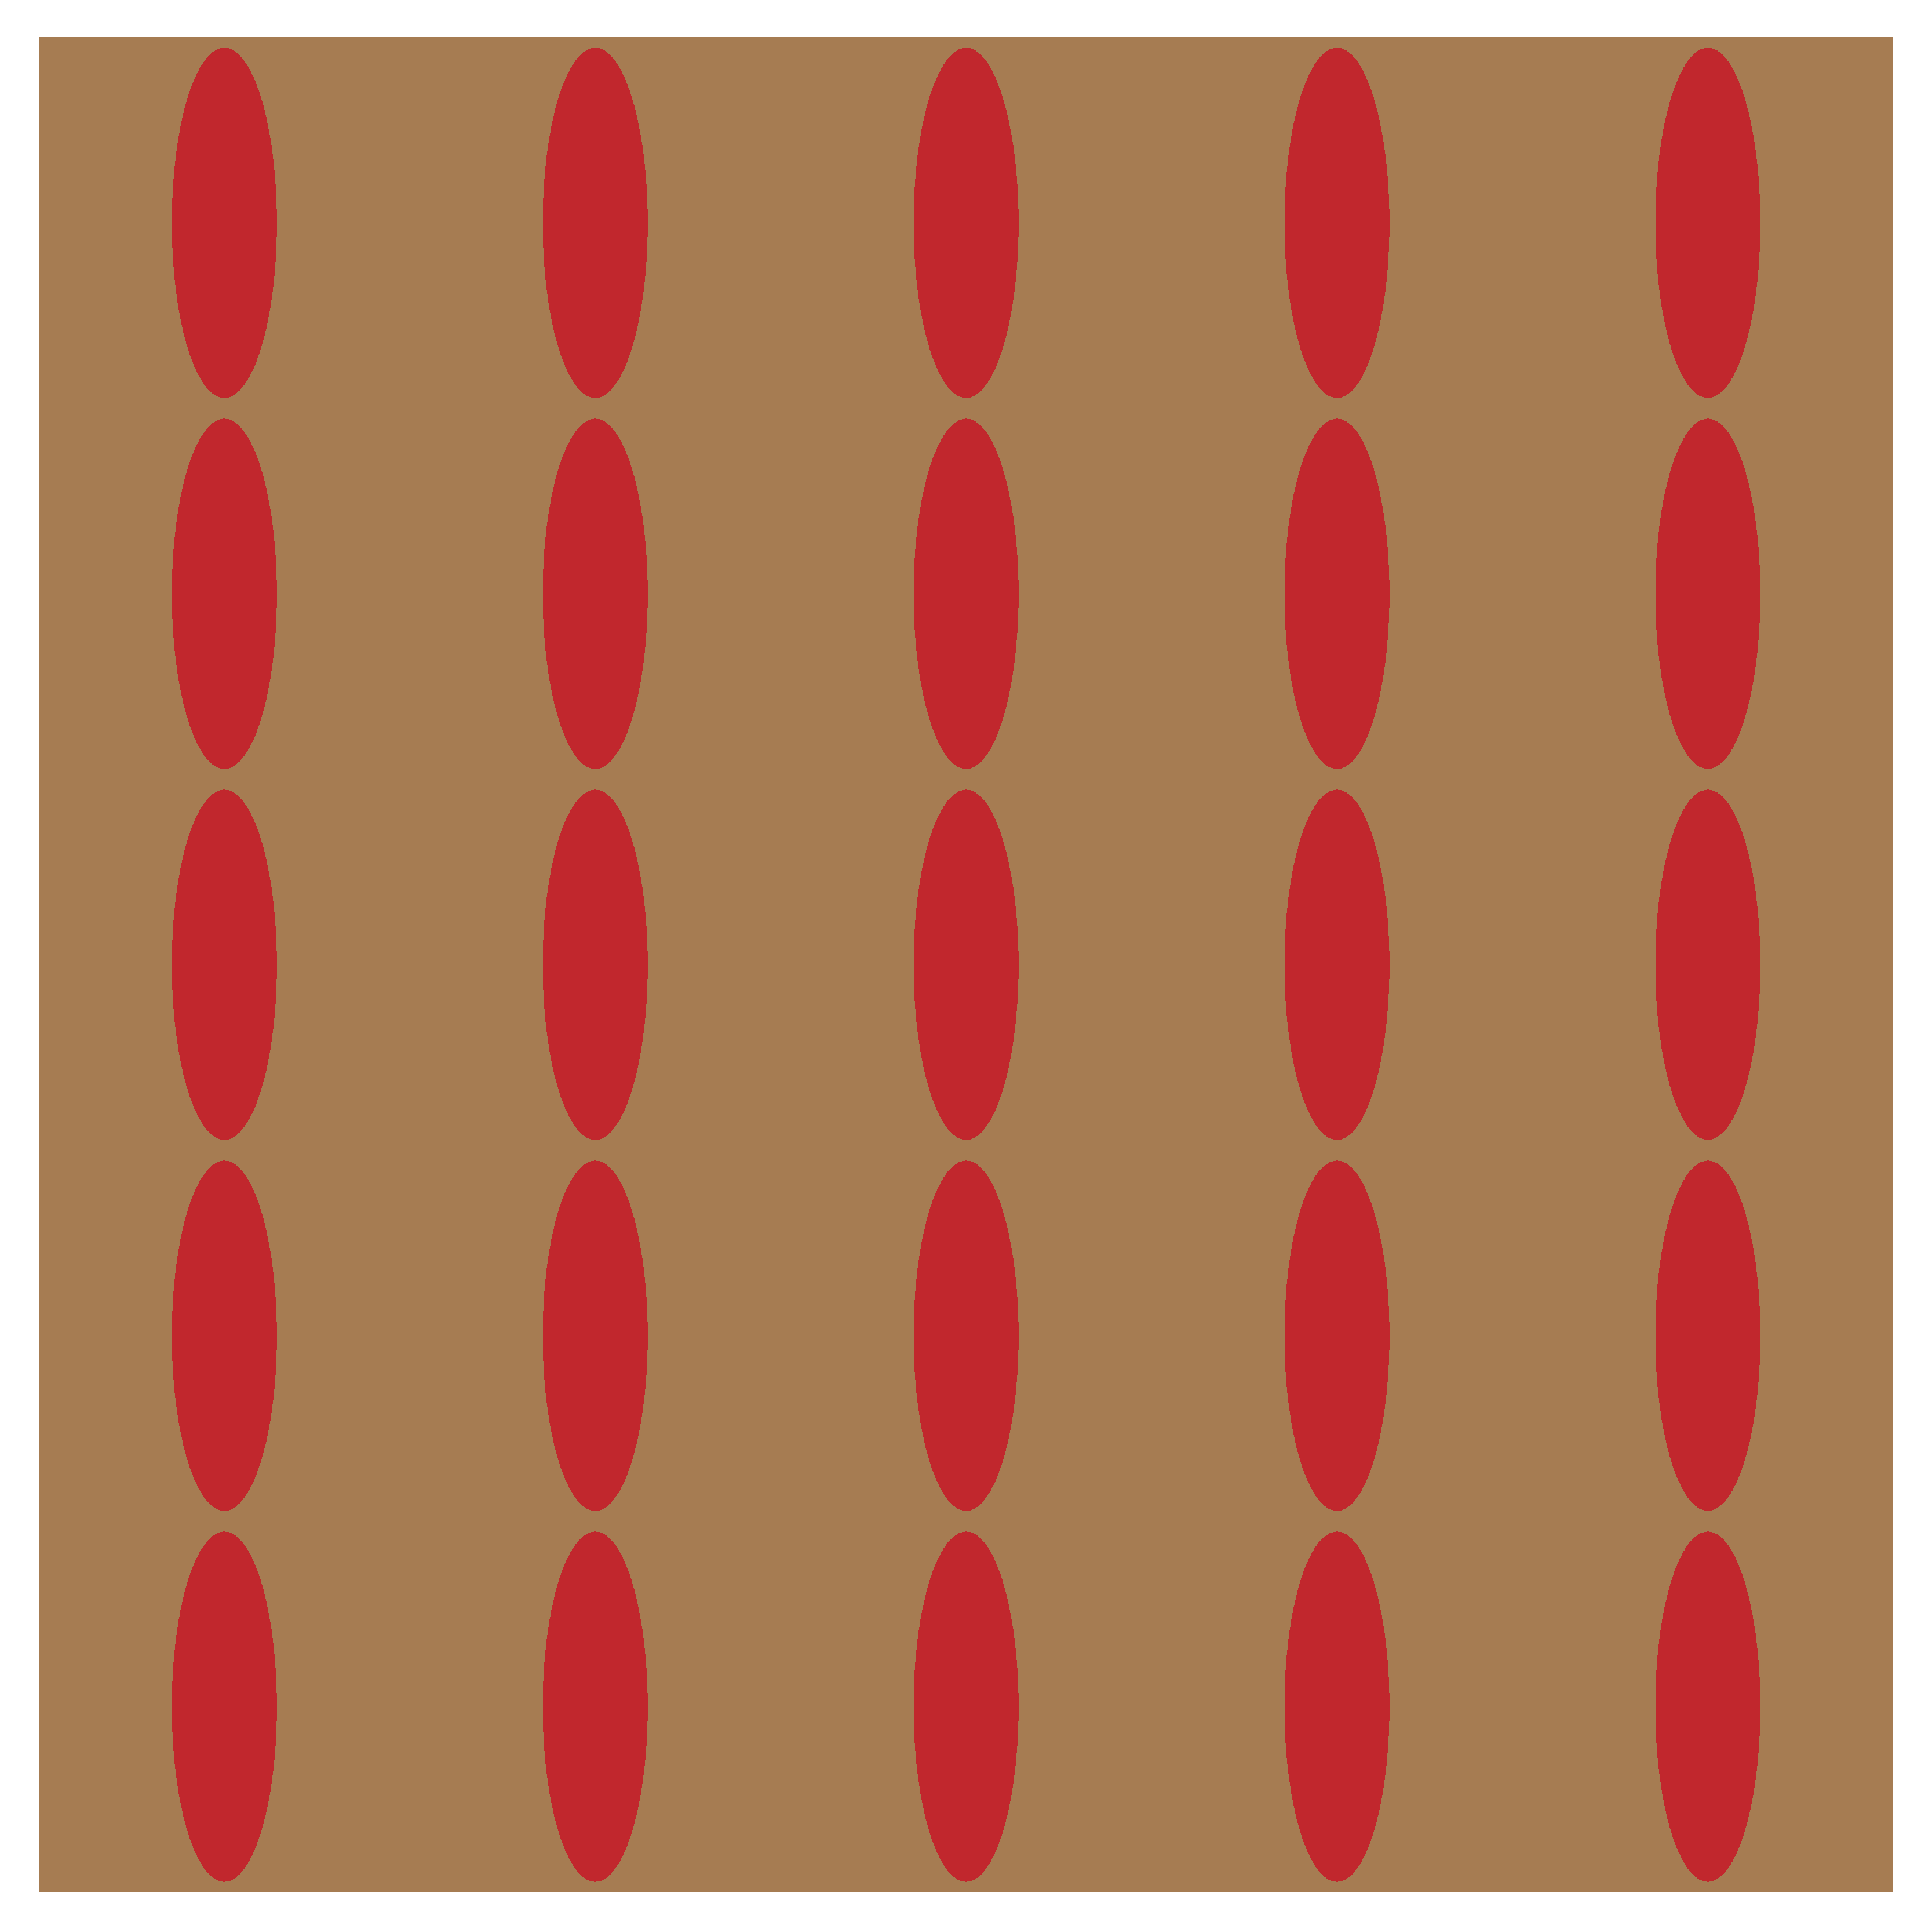
\includegraphics[width=\linewidth]{test_mesh_axR_0.3.png}
	\end{minipage} 
	\begin{minipage}[b]{0.19\linewidth}
		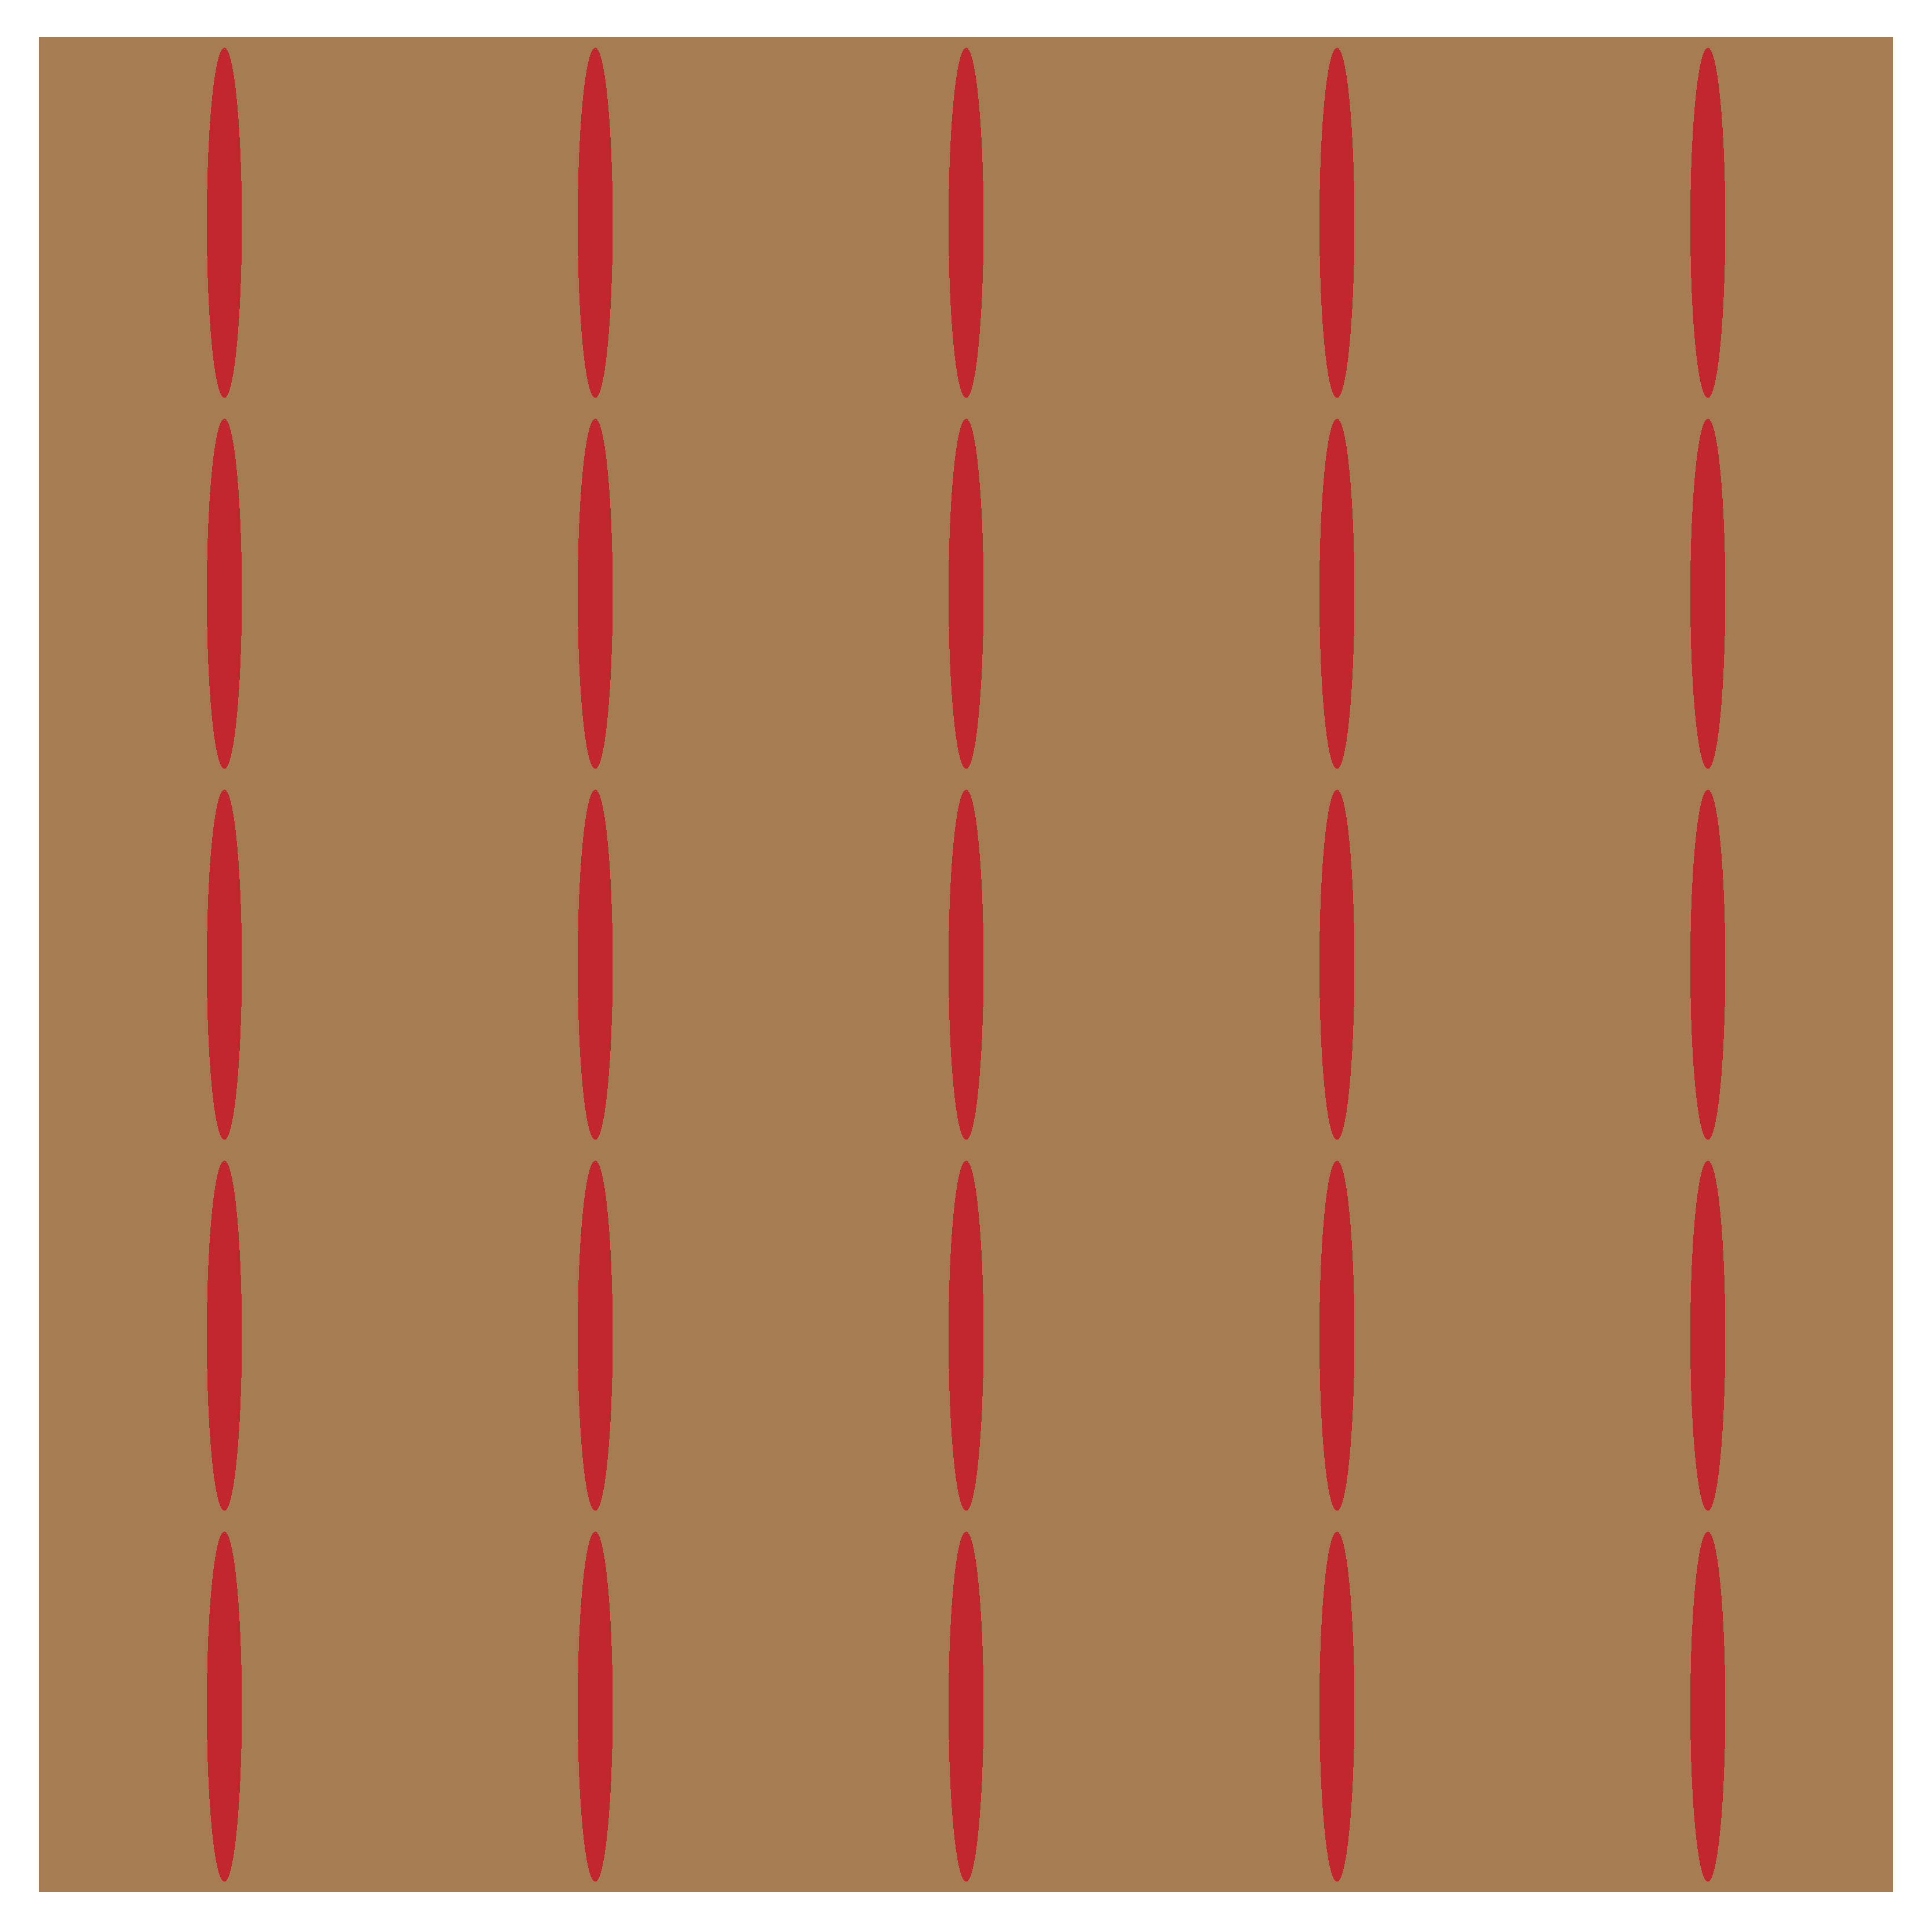
\includegraphics[width=\linewidth]{test_mesh_axR_0.1.png}
	\end{minipage} 
	
	\begin{minipage}[b]{0.19\linewidth}
		\footnotesize{$
			\begin{bmatrix}
				869.46 & 198.19 & 0.02 \\
				198.19 & 1857.50 & 0.01 \\
				0.03 & 0.01& 103.37 \\
			\end{bmatrix}
			$}
	\end{minipage}
	\begin{minipage}[b]{0.19\linewidth}
		\footnotesize{$
			\begin{bmatrix}
				1010.09 & 325.62 & 0.03 \\
				325.62 & 2883.80 & 0.01\\
				0.03 & 0.01 & 196.39 \\
			\end{bmatrix}
			$}
	\end{minipage}
	\begin{minipage}[b]{0.19\linewidth}
		\footnotesize{$
			\begin{bmatrix}
				1092.62 & 394.85 & 0.03\\
				394.85 & 3396.74 & 0.015 \\
				0.02 & 0.015 & 266.84 \\
			\end{bmatrix}
			$}
	\end{minipage}
	\begin{minipage}[b]{0.19\linewidth}
		\footnotesize{$
			\begin{bmatrix}
				1279.47 & 538.93 & 0.05 \\
				538.93 & 4416.36 & 0.02 \\
				0.05 & 0.02 & 483.75 \\
			\end{bmatrix}
			$}
	\end{minipage}
	\begin{minipage}[b]{0.19\linewidth}
		\footnotesize{$
			\begin{bmatrix}
				1462.51 & 653.01 & 0.62 \\
				653.01 & 5376.01 & 0.30 \\
				0.62 & 0.30 & 826.25 \\
			\end{bmatrix}
			$}
	\end{minipage} 
	
	\caption{Variazione della matrice di rigidezza al variare del rapporto assiale dei pori}
	\label{fig:geometry_variation} 
\end{figure*}

\label{sec:variazione_simmetria}

\begin{figure}[bt!] %% preferably at bottom or top of column

	\centering
	\def\svgwidth{0.9\linewidth}
	\input{var_geometr.pdf_tex}
	\caption{Relazione tra $C_{11}$, $C_{22}$ e $\operatorname{AxR}$ }
	\label{fig:geometric_variation}
\end{figure}




\begin{figure}[bt!] %% preferably at bottom or top of column
	\centering
	\def\svgwidth{0.9\linewidth}
	\input{variazione_Ebone.pdf_tex}
	\caption{Variazione di $\mathbb C_{11}$ al variare di $E_b$}\label{fig:var_Ebone}
\end{figure}

\begin{figure}[bt!] %% preferably at bottom or top of column
	\centering
	\def\svgwidth{0.9\linewidth}
	\input{variazione_Enarrow.pdf_tex}
	\caption{Variazione di $\mathbb C_{11}$ al variare di $E_m$}\label{fig:var_Emarrow}
\end{figure}



Le trabecole quindi rispondono al carico verticale posizionandosi prevalentemente lungo le linee di forza del carico e aumentano la loro densità e il loro spessore. Per indagare l'aumento delle proprietà materiali è stato considerato un RVE con pori variabili. Un modo semplice, ma accurato, di analizzare questo comportamento è quello di considerare pori ellittici. Introducendo pori ellittici la risposta dell'osso al carico verticale può essere interpretata come una riduzione del rapporto assiale e quindi un restringimento dell'ellisse lungo la direzione x. 

Le campagne di simulazione condotte mostrano diversi cambiamenti nella matrice di rigidezza e quindi nelle proprietà meccaniche. Partendo da un rapporto assiale molto basso, quindi un'ellisse molto schiacciata, si osserva un grande aumento nel parametro $C_{11}$ e un lieve aumento anche del parametro $C_{22}$ rispetto al caso di riferimento (\cref{sec:homogen}). Viene completamente meno la simmetria materiale e l'isotropia della matrice di rigidezza, segno che la risposta di rigidezza lungo la direzione del semidiametro maggiore è più grande di quella nella direzione del semidiametro maggiore. Questo rispecchia quanto produce l'osso con la sua risposta di rimodellamento. 

Con un rapporto assiale di $\operatorname{AxR}=0.1$ il coefficiente $C_{22}$ arriva a 1.462 GPa contro un $C_{11}=0.653$ GPa. Questa differenza del 44\% si riduce diminuendo il rapporto assiale. I due coefficienti convergono nel caso in cui il rapporto assiale tende a 1 ovvero nel caso in cui $C_{11}=C_{22}=C_{11}^{(om)}$. I limiti di Reuss e Voigt sono verificati in tutti i casi. I dati sono presenti in \cref{fig:geometry_variation} e\cref{fig:geometric_variation}. Nel diminuire il rapporto assiale il calo dei coefficienti di rigidezza segue un andamento lineare. Il coefficiente $C_{22}$ risente notevolmente di questo effetto mostrando una tasso di diminuzione del coefficiente $C_{11}$ con un andamento quasi costante. 

Rimane evidente come al diminuire del rapporto assiale, e quindi anche della volume fraction, sia i limiti di Reuss e Voigt sia l'omogenizzazione numerica mostrino il coefficiente maggiore tendere al coefficiente $C_{22}^{(b)}$ della sola matrice ossea pur rimanendo inferiore al 20\%.  

Lo stesso ragionamento può essere fatto nel caso contrario in cui malattie, come l'osteoporosi, portano ad una riduzione della massa ossea. Questo, rivisto come un aumento del rapporto assiale, mostra come l'osso trabecolare tende a ridurre le sue proprietà strutturali anche in zone dove precedentemente il rimodellamento osseo potrebbe aver apportato un precedentemente miglioramento strutturale (meno pori e maggior resistenza). Cambiamenti morfologici tra cui l'assottigliamento delle trabecole, aumento dello spazio inter-trabecolare e la perdita di connettività posso portare ad un calo drastico della resistenza fino al rischio di frattura vertebrale \citep{Ferguson:2003}.







\subsection{Estensione dell'area di indagine}
\label{sec:estensione}

\begin{figure*} 
\begin{center}
		\begin{minipage}[t]{0.24\linewidth}
\centerline{(a)}

	\end{minipage}
	\begin{minipage}[t]{0.24\linewidth}

\centerline{(b)}
	\end{minipage}
	\begin{minipage}[t]{0.24\linewidth}
\centerline{(c)}
	\end{minipage}
	\begin{minipage}[t]{0.24\linewidth}
\centerline{(d)}
	\end{minipage}
\hfill
	\begin{minipage}[c]{0.24\linewidth}
		\centering
	\def\svgwidth{\linewidth}
\input{distribution_100.pdf_tex}
						\newline
	\end{minipage}
	\begin{minipage}[c]{0.24\linewidth}
		\centering
	\def\svgwidth{\linewidth}
\input{distribution_300.pdf_tex}
	\newline
	\end{minipage}
	\begin{minipage}[c]{0.24\linewidth}
		\centering
			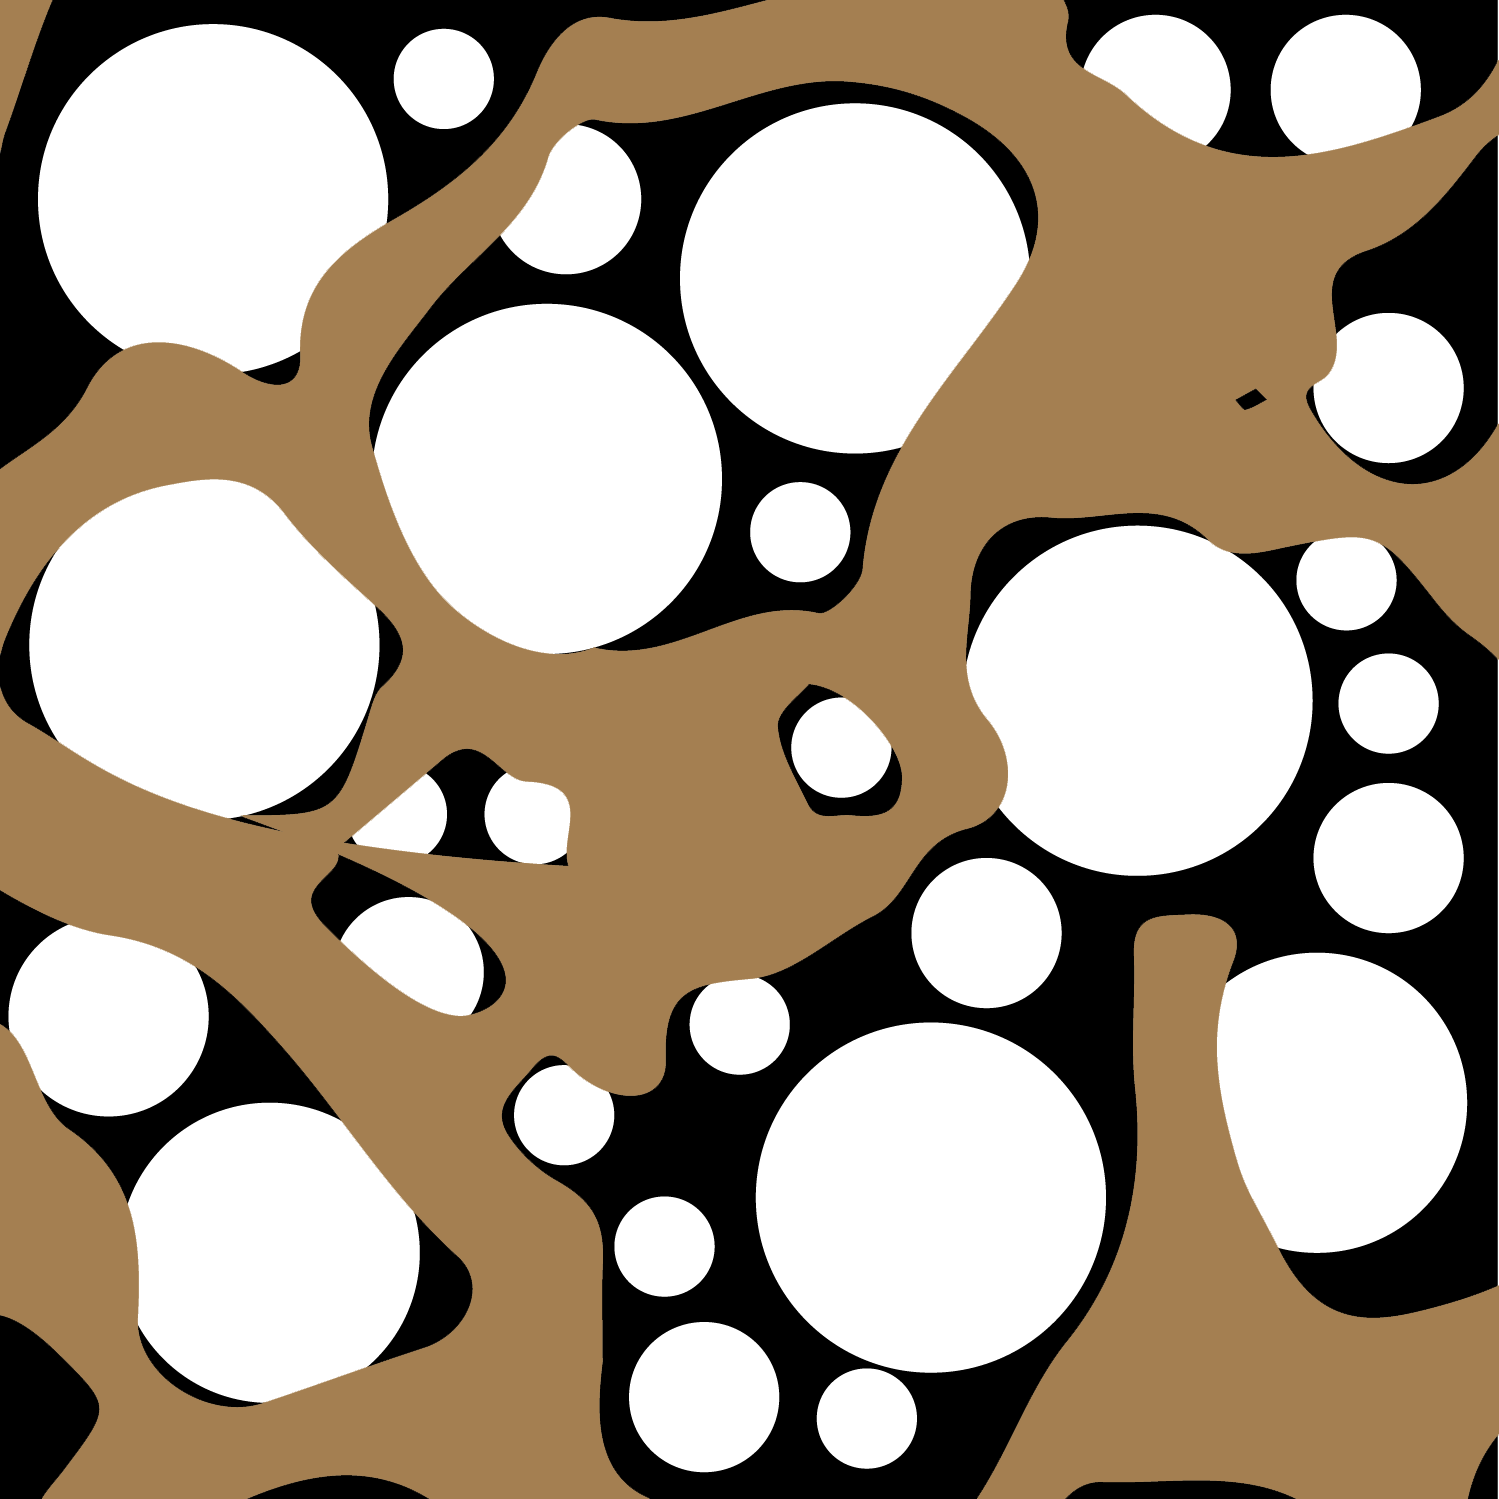
\includegraphics[width=\linewidth]{real_mesh_n1.png}
			\newline
	\end{minipage}
	\begin{minipage}[c]{0.24\linewidth}
		\centering
		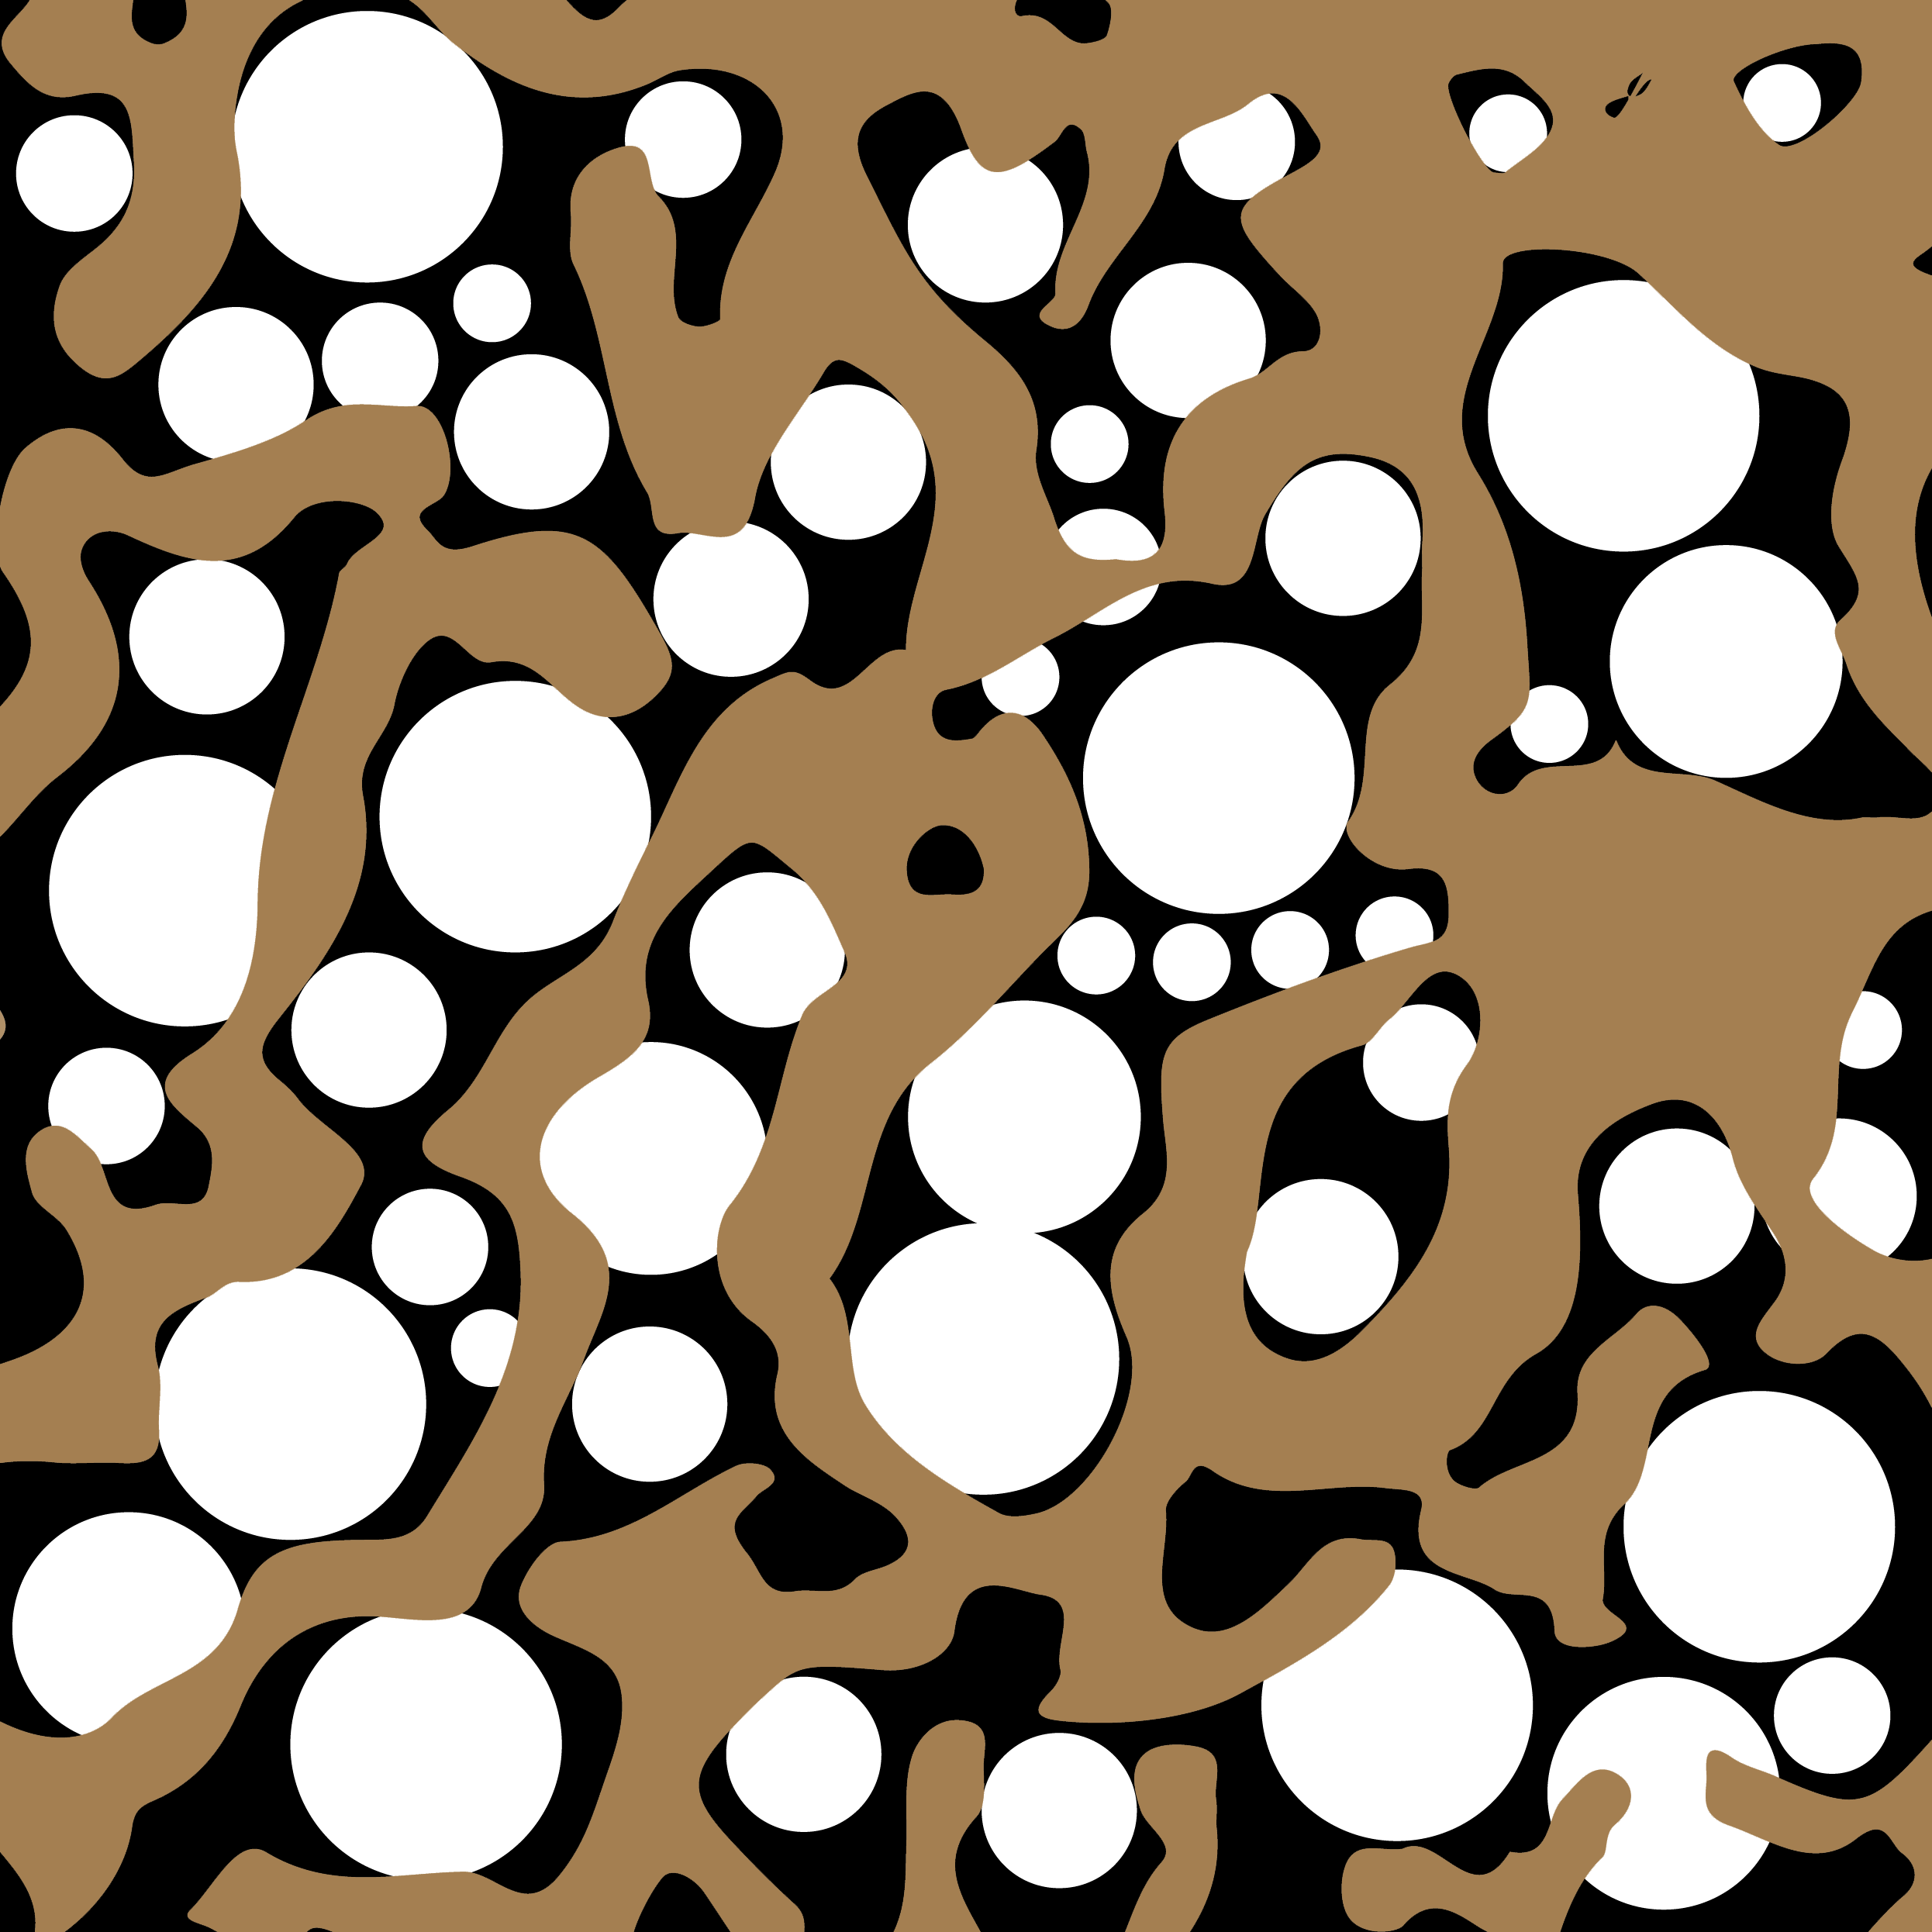
\includegraphics[width=\linewidth]{real_mesh_n2.png}
		\newline
	\end{minipage}
\hfill
	\begin{minipage}[b]{0.24\linewidth}
		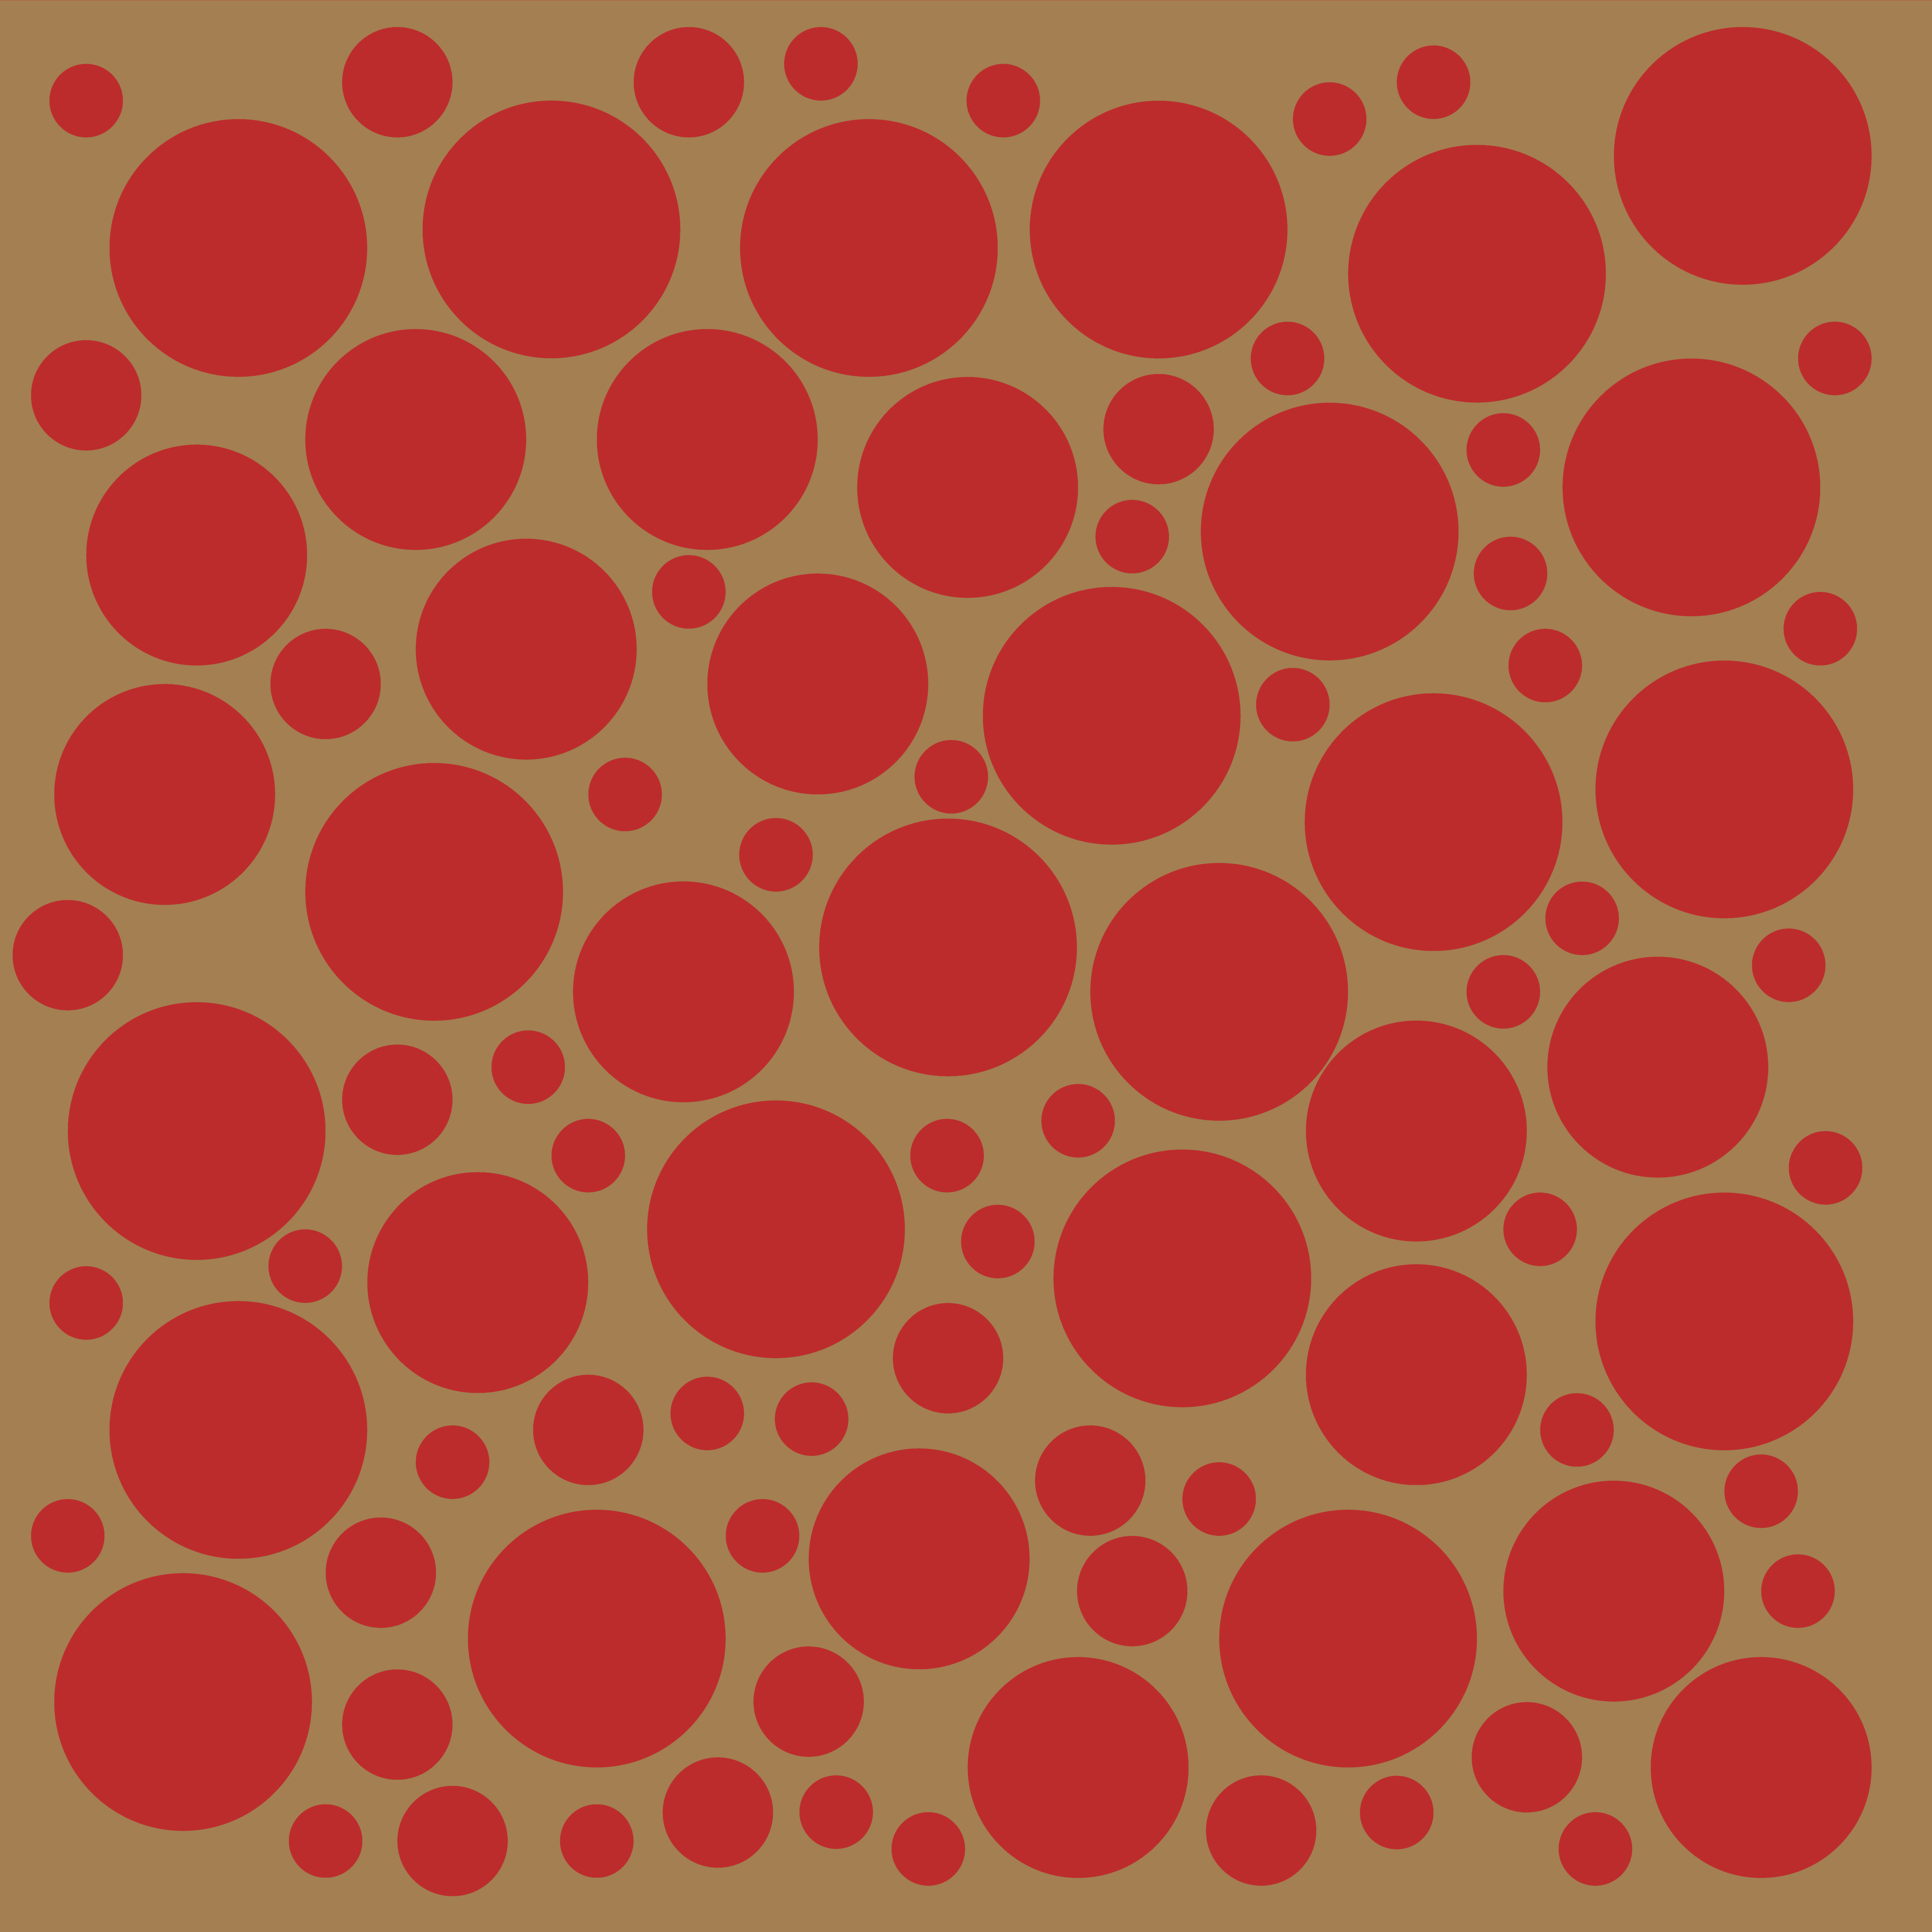
\includegraphics[width=\linewidth]{mesh_100.png}
				\newline
	\end{minipage} 
	\begin{minipage}[b]{0.24\linewidth}
		\includegraphics[width=\linewidth]{mesh_300.png}
						\newline
	\end{minipage} 
	\begin{minipage}[b]{0.24\linewidth}
	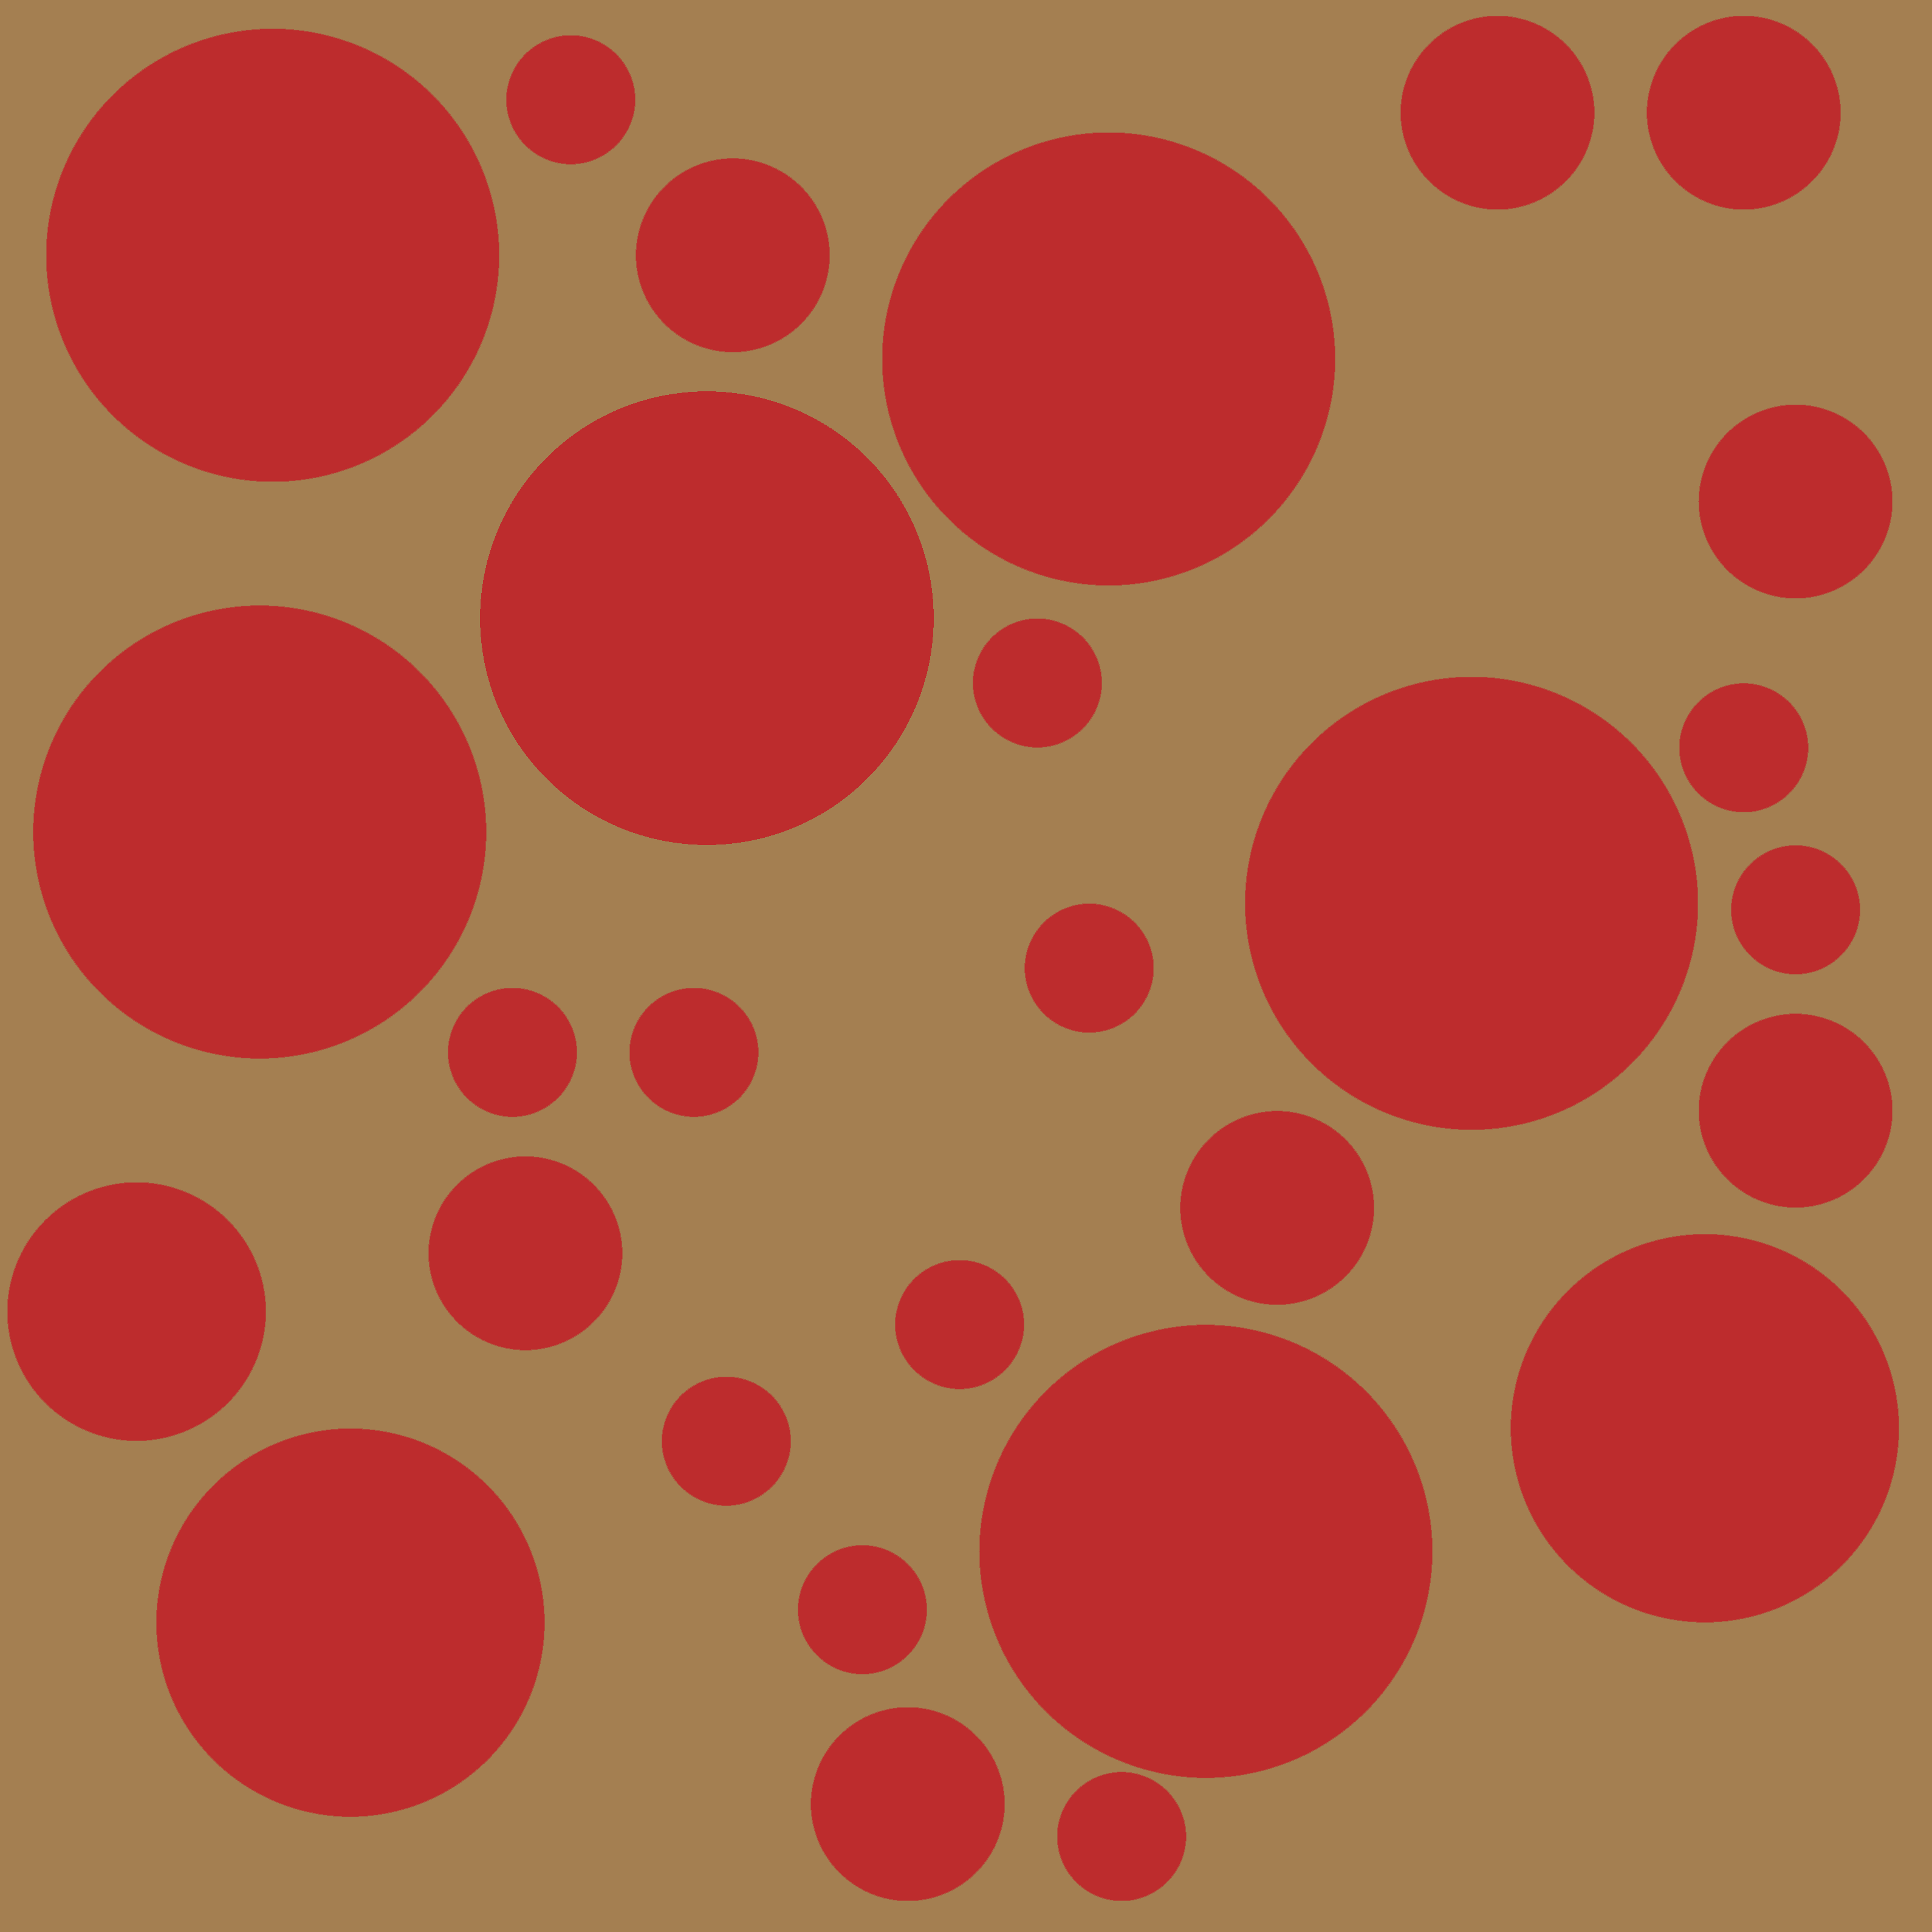
\includegraphics[width=\linewidth]{test_mesh_2.png}
				\newline
	\end{minipage}
	\begin{minipage}[b]{0.24\linewidth}
	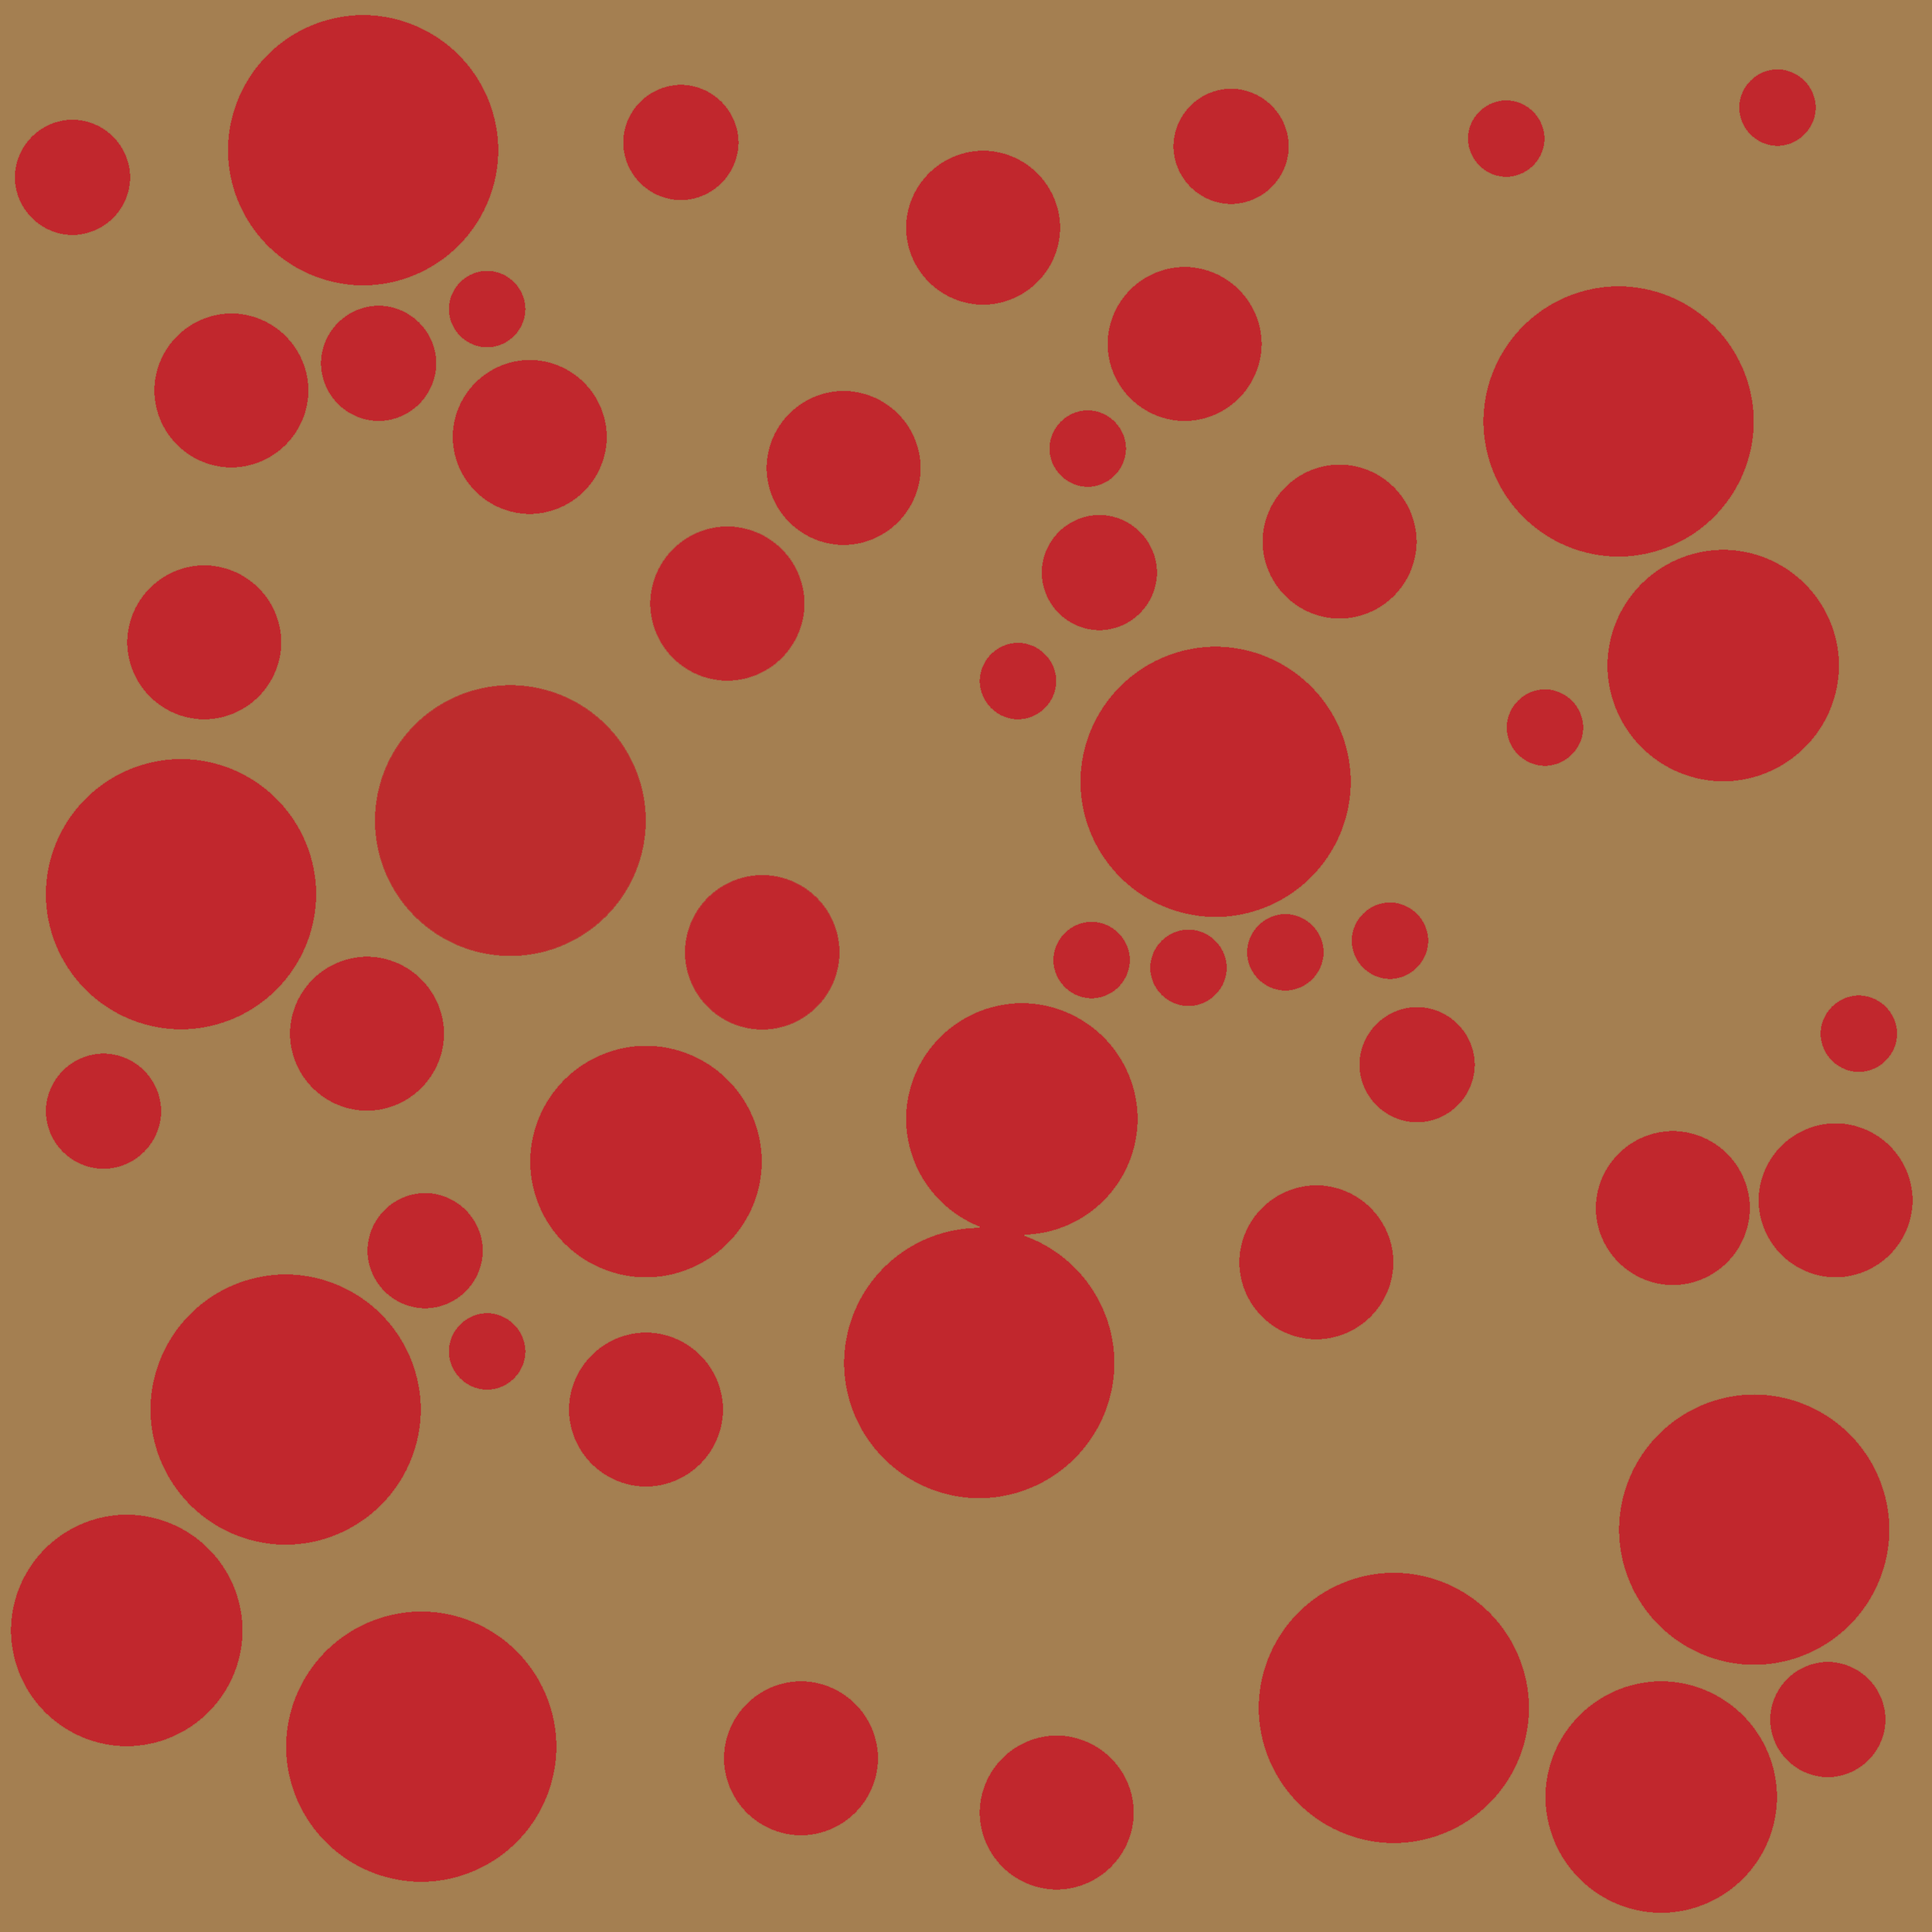
\includegraphics[width=\linewidth]{test_mesh_1.png}
					\newline
	\end{minipage} 
\hfill
	\begin{minipage}[b]{0.24\linewidth}
\centering
		\footnotesize{$
			\begin{bmatrix}
			 1034.17 & 411.96 & -11.69 \\
			411.96 & 1074.45 & -21.40 \\
			-11.67 & -21.41 & 224.12 \\
			\end{bmatrix}
			$}
	\end{minipage}
	\begin{minipage}[b]{0.24\linewidth}
\centering
		\footnotesize{$
			\begin{bmatrix}
			 959.28 & 439.22 & 0.29 \\
			439.21 & 995.56 & -11.64 \\
			0.29 & -11.63 & 209.55 \\
			\end{bmatrix}
			$}
	\end{minipage}
	\begin{minipage}[b]{0.24\linewidth}
\centering
		\footnotesize{$
			\begin{bmatrix}
			 1744.59 & 701.46 & 81.03 \\
			701.46 & 1649.60 & 49.05 \\
			81.03 & 49.05 & 540.63 \\
			\end{bmatrix}
			$}
	\end{minipage}
	\begin{minipage}[b]{0.24\linewidth}
\centering
		\footnotesize{$
			\begin{bmatrix}
			 2237.42 & 887.87 & 19.48 \\
			887.87 & 2394.87 & 71.54 \\
			19.48 & 71.54 & 690.04 \\
			\end{bmatrix}
			$}
	\end{minipage}
\hfill
	
	\caption{Variazione della regione di interesse. (a) introduzione di 100 pori con disposizione casuale; (b) introduzione di 300 pori con disposizione casuale; (c) introduzione di 28 pori su un RVE di lato $3$ mm; (d) introduzione di 52 pori su un RVE di lato $5$ mm.}
	\label{fig:area} 
\end{center}
\end{figure*}


Un'ulteriore indagine può essere quella di analizzare se e come varia la risposta meccanica variando la finestra di interesse. Avendo idealizzato un RVE simmetrico con pori simmetrici disposti su una griglia regolare è chiaro che, aumentando semplicemente il lato, si andrebbero ad includere semplicemente più pori. La volume fraction rimarrà la stessa così come la risposta meccanica. Anche se aumenta la somma delle tensioni queste vengono mediate su un area più grande e il loro rapporto, quindi la matrice di omogenizzazione, rimangono costanti. 

Lo studio si sposta alla su un RVE differente. I casi di interesse sono mostrati in \cref{fig:area}. L'analisi è divisa secondo due casistiche: 
\begin{itemize}
\item Analisi della risposta meccanica con una disposizione causale dei pori secondo una distribuzione nota  \citep{Doktor:2011}. 
\item Analisi della risposta meccanica con una distribuzione di pori ipotizzata a partire da un caso reale \citep{ESA:2005}.
\end{itemize}

Nell'analizzare i pori disposti secondo una distribuzione precisa vengono considerate diverse inclusioni di raggio fisso $\{0.1,\: 0.15,\: 0.2,\:0.03,\: 0.35\}$. Questi pori vengono disposti casualmente considerandone 100 (\cref{{fig:area}} (a)) o 300 (\cref{fig:area} (b)).

Si ottengono dei coefficienti della matrice di rigidezza $C_{11},C_{22}$ superiori al caso \cref{sec:homogen}. Questo in parte è dovuto ad una pore fraction minore, ovvero ad una presenza maggiore di matrice ossea che contribuisce ad aumentare la rigidezza complessiva. È interessante notare che il contributo della frazione volumetrica di pori si riflette in una matrice complessivamente più rigida lungo le direzioni principali anche se la struttura nel caso \cref{sec:homogen} sembra avere la matrice ossea lungo le direzioni di carico. 

Ad rafforzare queste conclusioni sono anche i risultati della precedente analisi (\cref{sec:variazione_simmetria}) . Confrontandoli con questi dati si vede come il fattore dominante rimane la pore fraction ma come aumenta la quantità di matrice ossea disposta lungo la direzione di carico aumenta la rigidezza in tale direzione. 

Nell'aumentare la regione di interesse vengono considerati 300 pori e viene aumentato il lato del RVE. Questo permette di includere un numero maggiore di pori e la loro distribuzione è tale da ridurre leggermente i coefficienti della matrice di rigidezza.

COMPLETA QUEST ODISCROS

PARLA DELLA PERDITA DI SIMMETRIA NELLA MATRICE

COMMENTA I COEFFICNENTI NU NU



COMMENTA SUI VALORI OTTENUTI RISPETTO QUELLI DELLA PRIMA OMOGENIZZAZIONE 



\subsection{Analisi caso specifica}


--> ESTENSIONE SU CASO SPECIFICA 

-->> DISTRIBUZIONE DI PORI 

--> MANTENENDO UNA PORE FRACTION DEL 60\%

\section{Parametri materiali}
\label{sec:variazioni_materiali}



Per il primo studio di omogenizzazione sono stati considerati dei parametri materiali medi tra quanto noto in letteratura. Tuttavia è noto anche che il modulo elastico delle strutture ossee può variare in relazione all'età o a particolari patologie. Diversi risultati mostrano che persone giovani hanno moduli di rigidezza più elevati delle persone anziane \citep{Cowin1}




\section{Conclusioni}

\section{???}


\section{Metodi}

\subsection{Elaborazione dell'immagine}

L'immagine presentata in figura \ref{fig:homogen_RVE}(a) è una ricostruzione 3D ottenuta con un algoritmo scritto ad hoc \citep{Mastrofini:21} a partire dalle singole slices (500-650) \citep{ESA:2005}. A seguire è stata selezionata la slice no. 650 che risulta essere quella a contrasto maggiore e soddisfa la frazione di pori \citep{CC21}. In particolare si può utilizzare il tool 
\texttt{Image Region Analyzer} in Matlab per averne conferma. Queste considerazioni, e soprattutto il volume 3D, hanno permesso di arrivare all'idealizzazione del volume di interesse presentata in  \cref{sec:RVE}

\subsection{Rappresentazione del volume di riferimento}
\label{sec:RVE_code}

Per la creazione dei fori viene considerata una griglia quadrata con $\sqrt{\text{N. fori}}$ per lato e viene generato un rettangolo esterno tale da garantire la volume fraction desiderata. Quindi viene generato anche un vettore contenente tutte le posizioni dei centri calcolate. Il calco viene effettuato con le funzioni \texttt{GeometryInitailization[]} e \texttt{GeometrySet[]}.

Vengono quindi creati e fori e assegnati i marker come identificato nello snippet \ref{code_rve}.  Un esempio di questo RVE in Figura \ref{fig:Mesh}.

Un calcolo più raffinato può essere fatto considerando la distribuzione del diametro dei pori \citep{Doktor:2011} e quindi creare i fori di diametro diverso rispettando la distribuzione. Chiaramente questo richiede un RVE con più inclusioni in modo da essere più rappresentativo. 

Per quanto riguarda la discretizzazione viene preso il valore ottimo tale da garantire un risultato sufficientemente accurato in tempi ridotti. Vedi \cref{sec:convergenza}.

Per la discretizzazione sono stati usati elementi T1LE, triangolari a 3 nodi con funzioni di forma lineari e una mappa isoparametrica.  

\begin{lstlisting}[language=Mathematica,caption=Generazione RVE,label=code_rve]
$\Omega$ext=Rectangle[{0,0},{Lx,Ly}];
$\Omega$=$\Omega$ext;
Do[$\Omega$=RegionDifference[
	$\Omega$,Disk[{centerx$\llbracket$i$\rrbracket$,centery$\llbracket$j$\rrbracket$},{Rc,Rc}]],
	{i,1,Ninclx},{j,1,Nincly}]
marker={{{Lx/100,Ly/100},1}};
Do[marker=Join[
	marker,{{{centerx$\llbracket$i$\rrbracket$,centery$\llbracket$j$\rrbracket$},2}}],
	{i,1,Ninclx},{j,1,Nincly}]
mesh=ToElementMesh[
$\Omega$,"RegionHoles"->None,"RegionMarker"->marker];	

\end{lstlisting}


\begin{figure}[b!]%[bt!] %% preferably at bottom or top of column
	\centering
	\includegraphics[width=\linewidth]{test_mesh_8.png}
	\caption{Mesh del volume rappresentativo con 756.787 DoF. I bordi appaiono neri e più spessi, questo è dovuto al refinement della mesh molto più fitta nei punti di bordo.}\label{fig:Mesh}
\end{figure}



\subsection{Codice}

\subsubsection{Condizioni al bordo}

Per impostare correttamente le condizioni al bordo in modo automatizzato è stato realizzato uno snippet ripetitivo con delle variabili di comando che permette di automatizzare la procedure. In particolare, volendo applicare una deformazione costante rispettivamente su $x$, $y$ o  di scorrimento è necessaria una mappa sulle condizioni di spostamento che permette di mappare ogni punto  nel valore desiderato. Si usano quindi la funzione \texttt{Function[{n, X, Y}, a*X + b*Y }, dove a seconda che sia nullo $a$ o $b$ lo spostamento sarà lineare rispettivamente in Y o in X. 

 Questo permette di impostare le condizioni sui quadrato bordi del quadrato mediante tre parametri $\{a,\:b,\:c\}$. Questi parametri vengono passati alla funzione \texttt{TEST[]} che provvede a mapparli come indicato nello snippet  \ref{code_displacem} andando ad impostare condizioni al contorno di tipo essenziale.  

Il test di omogenizzazione viene effettuato dalla funzione \texttt{Checkconvergence[]}. Questa funzione viene richiamata all'interno di un ciclo \texttt{Do} e nelle diverse iterazioni posso essere variati alcuni parametri come l'accuratezza della mesh, i parametri materiali o geometrici. 


\subsubsection{Verifica dei limiti superiore ed inferiore}

I limiti di Reuss e Voigt vengono calcolati tramite la funzione \texttt{VoigtReussTest[]} alla quale vengono passate le proprietà materiale dei singoli componenti insieme alla volume fraction. Quindi viene calcolata la matrice di rigidezza e di cedevolezza per un materiale isotropo e le approssimazioni di Reuss e Voigt. 

Vengono quindi verificati i due limiti verificando che $\mathbb C_{inf}=\mathbb C^{(om)}-\mathbb C_{Reuss} $ e $\mathbb C_{sup}=\mathbb C_{Voigt} - \mathbb C^{(om)}$ siano definite positive. In caso contrario il codice procede ma verrà comunicato che i limiti non sono verificati. 


\subsubsection{Variazioni proprietà}

Nel variare le proprietà materiali (\cref{sec:variazioni_materiali}) o della simmetria (\cref{sec:variazione_simmetria}) è stato sfruttata la funzione base di omogenizzazione (\texttt{Checkconvergence[]}) passandogli un vettore con i diversi parametri di interesse. Sono stati svolti test separati nel variare il modulo elastico della matrice ossea o dei pori.

Per variare le proprietà di simmetria è stato introdotto il rapporto assiale definito come il rapporto tra i due raggi: $\operatorname{AxR}=\frac{r_{x}}{r_y}$. 
Quindi tale parametri viene passato alla funzione \texttt{GeometrySet[]} per generare il RVE. 

\subsection{Estensione regione di interesse}

DESCRIVI IL NUOVO JOIN FATTO SU IMPLIIT REGION


\subsection{Analisi di convergenza}
\label{sec:convergenza}

Per effettuare l'analisi a convergenza è stata implementata una routine che ripete diverse volte l'omogenizzazione citata in \cref{sec:homogen} andando ad infittire la mesh. 

Vengono analizzati il modulo di $C_{11}$ e la norma della matrice $\| \mathbb C^{(om)}\|=\mathbb C^T\mathbb C$ e i loro valori normalizzati rispetto il valore vero. Viene assunto come valore vero quello dell'iterazione ultima, tale da considerare il risultato essere arrivato a convergenza. 
I risultati sui moduli estratti sono presenti nella Tabella \ref{tab:convergence} e nei due grafici dell'errore in \cref{fig:convergence} e in \cref{fig:convergence1}.

Analizzando i risultati è stato preso come valore ottimo quello ottenuto nell'iterazione 8 che presenta un errore rispetto il risultato ideale dello $0.11\%$ sul $\mathbb C_{11}$ e dello $0.23\%$ su $\|\mathbb C^{(om)}\|$a fronte di differenza di impegno computazionale del $83\%$. 


COMPLETA DA TEORIAAAAAAA




\begin{figure*}[bt!]
	\centering
	\begin{minipage}[b]{0.49\linewidth}

	\def\svgwidth{\linewidth}
	\input{test_data1.pdf_tex}
		\caption{Analisi dell'errore sul parametro $\mathbb C_{11}$}\label{fig:convergence}
	\end{minipage} 
	\begin{minipage}[b]{0.49\linewidth}
	\def\svgwidth{\linewidth}
	\input{test_data1.pdf_tex}
	\caption{Analisi dell'errore su $\|\mathbb C\|$}\label{fig:convergence1}
	\end{minipage} 
	\hfill
	\label{fig:convergenza} 
\end{figure*}



\begin{table}[bt!]
	\caption{Analisi di convergenza}\label{tab:convergence}
	\begin{tabular}{l c c c l}
		\toprule
\#&	$\mathbb C_{11}^{(om)}$ & $\| \mathbb C^{(om)}\| $ &DoF &  Time (s)\\
		\midrule

		
	1&		$845.289$ &$1450730 $ &$3368 $ &  $ 5.0625 $\\
			2&	$846.427$ &$145680 $& $3384$ &  $4.6719  $\\
			3&	$ 772.214$ &$1208530 $&$ 16874$  &  $ 8.9375 $\\
			4&$ 763.611$ &$ 1181190$&$ 39022$  &$ 14.875$   \\
			5&$ 759.333$ &$1168040 $&$ 253262$  & $ 64.0313$     \\
		6&	$ 759.333$ &$1168040 $& $ 253316$  &$ 60.5156$     \\
		7&	$758.829 $ &$1166450 $&$ 263104$   &$ 60.5781$     \\
		8&	$ 756.787$ &$ 1160210$&$ 453436$ &$ 94.8281 $     \\
		9&	$ 755.942$ &$1157590 $&$2800338 $  &  $ 507.0310$    \\
		10&	$755.903 $ &$ 1157470$&$ 3024312$  & $550.5780 $    \\
		\bottomrule
	\end{tabular}
\end{table}


\begin{lstlisting}[language=Mathematica,caption=Generazione RVE,label=code_displacem]
	SMTAddEssentialBoundary[Line[{{0, 0}, {0, Ly}}],
	1 -> Function[{n, X, Y}, b Y],
	2 -> Function[{n, X, Y}, c Y], 	"Set" -> True];
	SMTAddEssentialBoundary[Line[{{0, Ly}, {Lx, Ly}}],
		1 -> Function[{n, X, Y}, b*Ly + a*X],
		2 -> Function[{n, X, Y}, c*Ly + b*X], "Set" -> True];
	SMTAddEssentialBoundary[Line[{{Lx, Ly}, {Lx, 0}}], 
	1 -> Function[{n, X, Y}, a*Lx + b*Y],
	2 -> Function[{n, X, Y}, b*Lx + c*Y], "Set" -> True];
	SMTAddEssentialBoundary[Line[{{0, 0}, {Lx, 0}}],
	1 -> Function[{n, X, Y}, a*X],
	2 -> Function[{n, X, Y}, b*X], 	"Set" -> True];
\end{lstlisting}

\section{Disponibilità del codice e materiale aggiuntivo}

Tutto il codice, le immagini, file di processamento e risultati ottenuti sono disponibili alla repository online al link: \url{https://github.com/mastroalex/bone-homogenization}. 

Il codice per l'analisi di convergenza (\cref{sec:convergenza}) è presente nel file: \texttt{FEM->homogen->test\_analisi\_conv.nb}.

Il codice per la variazione delle proprietà di simmetria e la geometria del RVE (\cref{sec:variazione_simmetria}) è presente nel file:  \texttt{FEM->variazioni\_geometrie->test\_geometrie.nb}.

I codici per le variazioni delle proprietà materiali (\cref{sec:variazioni_materiali}) sono presenti nel file: \texttt{FEM->variazioni\_materiali->test\_materiali.nb}.


\subsection{Lista delle abbreviazioni}

\begin{itemize}
	\item RVE , rappresentative volume element 
	\item $\mathbb C^{(om)}$:,matrice di rigidezza ottenuta dall'omogenizzazione
	\item $\square_b$, parametri che fanno riferimento all'osso
	\item $\square_m$, parametri che fanno riferimento al midollo
	\item DoF, degrees of freedom
	\item $\operatorname{AxR}$, rapporto assiale nelle inclusioni ellissoidali
\end{itemize}
 


%% Specify your .bib file name here, without the extension
%\newpage
%\onecolumn

\newpage
\bibliography{paper-refs}




\end{document}
